\def\year{2021}\relax
%File: formatting-instructions-latex-2021.tex
%release 2021.2
\documentclass[letterpaper]{article} % DO NOT CHANGE THIS

\usepackage{aaai21}  % DO NOT CHANGE THIS             % TODO THIS PACKAGE SHOULD BE USED FOR ACTUAL CONFERENCE SUBMISSION!
% \usepackage{aaai21_no_copyright}  % DO NOT CHANGE THIS  % XXX TEMPORARILY DISABLED COPYRIGHT NOTICE FOR arXiv SUBMISSION!

\usepackage{times}  % DO NOT CHANGE THIS
\usepackage{helvet} % DO NOT CHANGE THIS
\usepackage{courier}  % DO NOT CHANGE THIS
\usepackage[hyphens]{url}  % DO NOT CHANGE THIS
\usepackage{graphicx} % DO NOT CHANGE THIS
\urlstyle{rm} % DO NOT CHANGE THIS
\def\UrlFont{\rm}  % DO NOT CHANGE THIS
\usepackage{natbib}  % DO NOT CHANGE THIS AND DO NOT ADD ANY OPTIONS TO IT
\usepackage{caption} % DO NOT CHANGE THIS AND DO NOT ADD ANY OPTIONS TO IT
\frenchspacing  % DO NOT CHANGE THIS
\setlength{\pdfpagewidth}{8.5in}  % DO NOT CHANGE THIS
\setlength{\pdfpageheight}{11in}  % DO NOT CHANGE THIS
%\nocopyright
%PDF Info Is REQUIRED.
% For /Author, add all authors within the parentheses, separated by commas. No accents or commands.
% For /Title, add Title in Mixed Case. No accents or commands. Retain the parentheses.
\pdfinfo{
/Title (PLGRIM: Hierarchical Value Learning for Large-scale Coverage in Unknown Environments)
% /Author (Sung-Kyun Kim*, Amanda Bouman*, Gautam Salhotra, David D. Fan, Kyohei Otsu, Joel Burdick, Ali-akbar Agha-mohammadi)
/Author Anonymous Authors  % XXX
/TemplateVersion (2021.2)
} %Leave this
% /Title ()
% Put your actual complete title (no codes, scripts, shortcuts, or LaTeX commands) within the parentheses in mixed case
% Leave the space between \Title and the beginning parenthesis alone
% /Author ()
% Put your actual complete list of authors (no codes, scripts, shortcuts, or LaTeX commands) within the parentheses in mixed case.
% Each author should be only by a comma. If the name contains accents, remove them. If there are any LaTeX commands,
% remove them.

% DISALLOWED PACKAGES
% \usepackage{authblk} -- This package is specifically forbidden
% \usepackage{balance} -- This package is specifically forbidden
% \usepackage{color (if used in text)
% \usepackage{CJK} -- This package is specifically forbidden
% \usepackage{float} -- This package is specifically forbidden
% \usepackage{flushend} -- This package is specifically forbidden
% \usepackage{fontenc} -- This package is specifically forbidden
% \usepackage{fullpage} -- This package is specifically forbidden
% \usepackage{geometry} -- This package is specifically forbidden
% \usepackage{grffile} -- This package is specifically forbidden
% \usepackage{hyperref} -- This package is specifically forbidden
% \usepackage{navigator} -- This package is specifically forbidden
% (or any other package that embeds links such as navigator or hyperref)
% \indentfirst} -- This package is specifically forbidden
% \layout} -- This package is specifically forbidden
% \multicol} -- This package is specifically forbidden
% \nameref} -- This package is specifically forbidden
% \usepackage{savetrees} -- This package is specifically forbidden
% \usepackage{setspace} -- This package is specifically forbidden
% \usepackage{stfloats} -- This package is specifically forbidden
% \usepackage{tabu} -- This package is specifically forbidden
% \usepackage{titlesec} -- This package is specifically forbidden
% \usepackage{tocbibind} -- This package is specifically forbidden
% \usepackage{ulem} -- This package is specifically forbidden
% \usepackage{wrapfig} -- This package is specifically forbidden
% DISALLOWED COMMANDS
% \nocopyright -- Your paper will not be published if you use this command
% \addtolength -- This command may not be used
% \balance -- This command may not be used
% \baselinestretch -- Your paper will not be published if you use this command
% \clearpage -- No page breaks of any kind may be used for the final version of your paper
% \columnsep -- This command may not be used
% \newpage -- No page breaks of any kind may be used for the final version of your paper
% \pagebreak -- No page breaks of any kind may be used for the final version of your paperr
% \pagestyle -- This command may not be used
% \tiny -- This is not an acceptable font size.
% \vspace{- -- No negative value may be used in proximity of a caption, figure, table, section, subsection, subsubsection, or reference
% \vskip{- -- No negative value may be used to alter spacing above or below a caption, figure, table, section, subsection, subsubsection, or reference

% \setcounter{secnumdepth}{0} %May be changed to 1 or 2 if section numbers are desired.
\setcounter{secnumdepth}{2} %May be changed to 1 or 2 if section numbers are desired.


%%%%%%%%%%%%%%%%%%%%%%%%%%%%%%%%%%%%%%%
%%%%%%%%%%%%%%%%%%%%%%%%%%%%%%%%%%%%%%%

\usepackage[utf8]{inputenc}
\usepackage[T1]{fontenc}
\usepackage{graphicx}
\usepackage{float}
\usepackage{xcolor}
\usepackage[normalem]{ulem}
\usepackage{subfig}

\usepackage{amsmath}
\usepackage{amsfonts}
\usepackage{amssymb}
\usepackage{mathtools}
\usepackage{todonotes}
\usepackage{enumitem}
\usepackage{multicol}
\usepackage{comment}
% \usepackage[noend]{algpseudocode} % this breaks my algorithm box

\usepackage{tikzpagenodes}

% \usepackage[
%   subtle
%   %moderate
% ]{savetrees}

\usepackage{algorithm,algorithmic}

\newcommand{\ph}[1]{{\textbf{#1}:}} % paragraph header
% \newcommand{\phdone}[1]{{\textbf{#1}:}} % (invisible) paragraph header
\newcommand{\phdone}[1]{} % (invisible) paragraph header
\newcommand{\ncomment}[1]{}
% \newcommand{\todo}[1]{{\color{red} #1 }} % Tasks to do
\newcommand{\note}[1]{{\color{cyan} NOTE: #1 }}
\newcommand{\hn}[1]{{\color{orange} NOTE: (Henry) #1 }}
\newcommand{\gautam}[1]{{\color{cyan}Gautam: #1 }}
% \newcommand{\gautam}[1]{{\color{cyan}}}
\newcommand{\maximize}{\mathop{\mathrm{maximize}}}
\newcommand{\argmax}{\mathop{\mathrm{argmax}}}
\newcommand{\argmin}{\mathop{\mathrm{argmin}}}

\newcommand{\ali}[1]{{\color{blue} #1 }}
%\newcommand{\ali}[1]{} % to remove Ali's comments

%%%%%%%%%%%%%%%%%%%%%%%%%%%%%%%%%%%%%%%
%%%%%%%%%%%%%%%%%%%%%%%%%%%%%%%%%%%%%%%



% The file aaai21.sty is the style file for AAAI Press
% proceedings, working notes, and technical reports.
%

% Title

% Your title must be in mixed case, not sentence case.
% That means all verbs (including short verbs like be, is, using,and go),
% nouns, adverbs, adjectives should be capitalized, including both words in hyphenated terms, while
% articles, conjunctions, and prepositions are lower case unless they
% directly follow a colon or long dash

\title{
    % PLGRIM: Hierarchical Value Learning for Large-scale \\Coverage in Unknown Environments
    PLGRIM: Hierarchical Value Learning for \\Large-scale Exploration in Unknown Environments
}
\author{
    Anonymous Authors \\  % XXX
    % Sung-Kyun Kim,\thanks{These authors contributed equally to this work.}\textsuperscript{\rm 1}
    % Amanda Bouman,$^{*}$\textsuperscript{\rm 2}
    % Gautam Salhotra,\textsuperscript{\rm 3}
    % David D. Fan,\textsuperscript{\rm 1} \\
    % Kyohei Otsu,\textsuperscript{\rm 1}
    % Joel Burdick,\textsuperscript{\rm 2}
    % Ali-akbar Agha-mohammadi\textsuperscript{\rm 1} \\
}
\affiliations{
    % Affiliation  % XXX
    % \textsuperscript{\rm 1}
    % NASA Jet Propulsion Laboratory,
    % California Institute of Technology
    % \\ \{sung.kim,
    % david.d.fan,
    % kyohei.otsu,
    % aliagha\}@jpl.nasa.gov
    % % \\ aliakbar.aghamohammadi@jpl.nasa.gov
    % \\
    % \textsuperscript{\rm 2}
    % Department of Mechanical and Civil Engineering,
    % California Institute of Technology
    % \\ abouman@caltech.edu,
    % jwb@robotics.caltech.edu
    % \\
    % \textsuperscript{\rm 3}
    % Department of Computer Science,
    % University of Southern California
    % \\ salhotra@usc.edu
}
% \author{
%     %Authors
%     % All authors must be in the same font size and format.
%     Written by AAAI Press Staff\textsuperscript{\rm 1}\thanks{With help from the AAAI Publications Committee.}\\
%     AAAI Style Contributions by Pater Patel Schneider,
%     Sunil Issar,  \\
%     J. Scott Penberthy,
%     George Ferguson,
%     Hans Guesgen,
%     Francisco Cruz,
%     Marc Pujol-Gonzalez
%     \\
% }
% \affiliations{
%     %Afiliations
%     \textsuperscript{\rm 1}Association for the Advancement of Artificial Intelligence\\
%     %If you have multiple authors and multiple affiliations
%     % use superscripts in text and roman font to identify them.
%     %For example,
%
%     % Sunil Issar, \textsuperscript{\rm 2}
%     % J. Scott Penberthy, \textsuperscript{\rm 3}
%     % George Ferguson,\textsuperscript{\rm 4}
%     % Hans Guesgen, \textsuperscript{\rm 5}.
%     % Note that the comma should be placed BEFORE the superscript for optimum readability
%
%     2275 East Bayshore Road, Suite 160\\
%     Palo Alto, California 94303\\
%     % email address must be in roman text type, not monospace or sans serif
%     publications21@aaai.org
%
%     % See more examples next
% }
\iffalse
%Example, Single Author, ->> remove \iffalse,\fi and place them surrounding AAAI title to use it
\title{My Publication Title --- Single Author}
\author {
    % Author
    Author Name \\
}

\affiliations{
    Affiliation \\
    Affiliation Line 2 \\
    name@example.com
}
\fi

\iffalse
%Example, Multiple Authors, ->> remove \iffalse,\fi and place them surrounding AAAI title to use it
\title{My Publication Title --- Multiple Authors}
\author {
    % Authors
    First Author Name,\textsuperscript{\rm 1}
    Second Author Name, \textsuperscript{\rm 2}
    Third Author Name \textsuperscript{\rm 1} \\
}
\affiliations {
    % Affiliations
    \textsuperscript{\rm 1} Affiliation 1 \\
    \textsuperscript{\rm 2} Affiliation 2 \\
    firstAuthor@affiliation1.com, secondAuthor@affilation2.com, thirdAuthor@affiliation1.com
}
\fi
\begin{document}

\maketitle

\begin{abstract}
% In order for a mobile robot to achieve higher levels of autonomy in unknown environments, it must account for uncertainty in sensor measurements, localization, and hazards assessment, as well as robot's own action execution.
In order for a robot to explore an unknown environment autonomously, it must account for uncertainty in sensor measurements, hazard assessment, localization, and motion execution.
Making decisions for maximal reward in a stochastic setting requires learning values and constructing policies over a belief space, i.e., probability distribution of the robot-world state.
Value learning over belief spaces suffer from computational challenges in high-dimensional spaces, such as large spatial environments and long temporal horizons for exploration. % required in many real-world missions. %An effective planner must be computationally efficient and handle time constraints without severely impacting the optimality of the solution.
At the same time, it should be adaptive and resilient to disturbances at run time in order to ensure the robot's safety, as required in many real-world applications.
% This work proposes a scalable value learning framework, PLGRIM (Planning at Local-Global levels with Robust Information roadMaps), that bridges the gap between \textit{(i)} local, risk-aware resilience and \textit{(ii)} global, reward seeking mission objectives.
This work proposes a scalable value learning framework, PLGRIM (Probabilistic Local and Global Reasoning on Information roadMaps), that bridges the gap between \textit{(i)} local, risk-aware resilience and \textit{(ii)} global, reward-seeking mission objectives.  
% Another one: PLGRIM (Probabilistic Local and Global Reasoning using Information Maps)
By leveraging hierarchical belief space planners with information-rich graph structures, PLGRIM can address large-scale exploration problems while providing locally near-optimal coverage plans. % within a receding horizon. \gautam{what do you mean 'within a receding horizon'? Maybe use 'near-optimal finite-horizon coverage plans'?}
% @Sung you can also say locally near-optimal coverage plans with a receding horizon  maybe?
% @Gautam Or can we say 'for a receding horizon'?
% Yes sure
% We take samples of the belief space in order to construct a graph structure that encodes mission and environment-related information, which we call an Information Roadmap (IRM).  
PLGRIM is a step toward enabling belief space planners %aims at bridging the gap between %pushes the boundaries of the state-of-art in 
on physical robots operating in unknown and complex environments. 
% As a concrete example, we demonstrate the performance of PLGRIM on Boston Dynamics' quadruped Spot robot operating in lava tubes.
%and demonstrate its performance as the planning core of the NeBula 2.0 autonomy framework. NeBula 1.0 (prior to PLGRIM integration) framework and the adopted hardware in this demonstration have contributed to winning first place in the 2020 DARPA Subterranean Challenge, Urban Circuit.
We validate our proposed framework with a high-fidelity dynamic simulation in diverse environments and with physical hardware, Boston Dynamics' Spot robot, in a lava tube.

%In  particular,  we  will  discuss  the  behaviors  andcapabilities  which  emerge  from  the  integration  of  the  auton-omy  architecture  NeBula  (Networked  Belief-aware  PerceptualAutonomy)   with   next-generation   mobility   systems.   We   willdiscuss  the  hardware  and  software  challenges,  and  solutionsin mobility, perception, autonomy, and wireless networking, aswell  as  lessons  learned  and  future  directions.  

%our framework for autonomous exploration in simulation with large environments with rough terrains and complex topology.
% We demonstrate our framework in team CoSTAR's participation in the DARPA Subterranean Challenge, in which teams compete to autonomously search for artifacts in large, unknown, GPS-denied environments.
\end{abstract}


%%%%%%%%%%%%%%%%%%%%%%%%%%%%%%%%%%%%%%%%%%%%%%%%%%%%%%%%%%%%%%%%%%%%%%%%%%%%%%%%
\section{Introduction}

\phdone{High-level mission}
Consider a large-scale coverage mission in an unknown environment, in which a robot is tasked with exploring and searching a GPS-denied unknown area, under given time constraints. Essential elements of an autonomy architecture needed to realize such a mission include creating a map of the environment, accurately predicting risks, and planning motions that can meet the coverage and time requirements while minimizing risks.  In such an architecture, quantifying and planning over uncertainty is essential for creating robust, intelligent, and optimal behaviors.


% \begin{figure}[t]
%   \centering
% %   \includegraphics[width=.48\columnwidth]{figures/firstpage_v2.png}
%   \includegraphics[width=.7\columnwidth,trim={0 0 0 11.0cm},clip]{figures/firstpage_v2.png}
%   \caption{ %The top figure shows a portion of the course in the Urban Circuit of the DARPA Subterranean Challenge. The blue line highlights two neighboring rooms joined by a narrow passage. CoSTAR efficiently explored both rooms by planning on the IRM. 
%   IRM and lattice visualization during an autonomous exploration mission.}
%   \label{fig:firstPage}
% \end{figure}

% \begin{figure}[t!]
%   \centering
%   \includegraphics[width=.4\columnwidth]{figures/graph-lattice-map.pdf}
%   \caption{Visualization of hierarchical Information RoadMaps (IRMs).}
%   \label{fig:firstPage}
% \end{figure}
% \begin{figure}[t!]
%   \centering
%   \includegraphics[width=.6\columnwidth]{figures/SystemOverview.png}
%   \caption{[WIP] System overview}
%   \label{fig:system_overview}
% \end{figure}
% \begin{figure}[t!]
%   \centering
%   \subfloat[System diagram (replace with real robot in cave?)\label{fig:system_overview}]{
%     \includegraphics[width=.85\columnwidth,trim={0 5.5cm 9.0cm 0},clip]{figures/SystemOverview.pdf}
%   }
%   % \quad
%   \\
% %   \subfloat[Visualization of hierarchical IRMs]{%
% %   \subfloat[Hierarchical IRMs]{%
%   \subfloat[Graph/Lattice IRMs\label{fig:irms}]{%
%     \includegraphics[width=.40\columnwidth,trim={0 7cm 16cm 0},clip]{figures/graph-lattice-map.pdf}
%   }
%   \caption{Overall framework of hierarchical Information RoadMaps (IRMs) and POMDP planners.}
%   \label{fig:firstPage}
% \end{figure}

% \begin{figure}[t!]
%   \centering
%   \includegraphics[width=1\columnwidth]{figures/hierarchy_labels.png}
%   \caption{[TODO] Hierarchical Information RoadMaps (IRMs) for large-scale exploration in unknown environments.}
%   \label{fig:firstPage}
% \end{figure}


\begin{figure}[t!]
\centering
    \begin{tikzpicture}
    \node[anchor=south west,inner sep=0] (image) at (0,0) {\includegraphics[width=1\columnwidth]{figures/hierarchy_labels_spot.png}};
	    \begin{scope}[x={(image.south east)},y={(image.north west)}]
	    	
	    	% Annotations 
	    	\node [font=\scriptsize,above left,align=right,black] at (0.93,0.79) {Local IRM}; %{Lattice IRM};
	    	\node [font=\scriptsize,above left,align=right,black] at (0.7,0.54) {Riskmap}; %{Graph IRM};
	    	\node [font=\scriptsize,above left,align=right,black] at (0.38,0.08) {Pose Graph};
	    	\node [font=\scriptsize,above left,align=right,black] at (0.17,0.29) {Global IRM};

	    \end{scope}
	\end{tikzpicture}	
  \caption{Hierarchical Information RoadMaps (IRMs) for large-scale exploration in unknown environments. [TODO: Add more explanation]} \label{fig:IRMs} 
\end{figure}




% \begin{figure}[t!]
%   \centering
%   \includegraphics[width=.6\columnwidth,trim={0 0 0 1.0cm},clip]{figures/SystemOverview.png}
%   \caption{System diagram of the overall PLGRIM framework.}
%   \label{fig:system_overview}
% \end{figure}

% \begin{figure}[t!]
%   \centering
%   \includegraphics[width=.6\columnwidth]{figures/sketch_hierarchical_belief_space.png}
%   \caption{Illustration. [TODO] Visualize the planned path in each level.}
%   \label{fig:illustration}
% \end{figure}


From value learning perspective, a coverage planning problem in an unknown space can be considered an active learning problem over the robot's belief, where belief is defined as the probability distributions over all possible joint robot-world states.
%
The objective is to find the best action sequence that maximizes the accumulated reward over time.  The agent must accumulate data to incrementally build a model of its environment, and must understand the effects of its actions on the quality and quantity of data it collects.

\phdone{Problem description--POMDP perspective}
Since the agent's future actions affect its belief of the world and robot state, this coverage problem is fundamentally a Partially Observable Markov Decision Process (POMDP) problem.
%A POMDP is a principled formalization of 
%a sequential decision making process under motion and sensing uncertainty.
The agent employs the underlying intrinsic model of the sequential action-observation process under uncertainty, so that it can %(asymptotically) converge to the optimal solution in a more 
expand its search structure over the space and learn the value in a more sample-efficient manner than model-free learning approaches.
[In addition, its non-myopic reasoning provides better performance than one-step look-ahead frontier selection approaches.]

\phdone{Gap in the state-of-the-art}
Belief value learning in POMDP setting suffers from the curse of dimensionality \cite{KLC98} and curse of history \cite{Pineau03}. Many powerful methods are extending the spatial and temporal horizons of POMDPs with varying degrees of efficiency and accuracy (e.g., \cite{silver2010monte,somani2013despot,bonet1998learning,kim2019pomhdp}). In this paper, we deal with exploration problems with very long time horizons (> 1 hour), large spatial extents (> 10 km$^2$), and high dimensional belief states (including beliefs on the state of the environment), that exacerbates the curses of history and dimensionality when planning robot behaviors over the belief space.
%

\phdone{Contributions}
To address this problem, we introduce several key spatial and temporal approximations of the robot policy space to enable computational tractability while constructing an online and real-time solver.
%search space.  This decomposition allows us to approximately solve the optimization problem in a computationally tractable manner.  
Spatially, we decompose the belief space into task-relevant partitions of the space,
%into a robot and task-relevant graph structure 
enriched with environment map estimates. %, which reduces our search space for good policies, 
The partitioning structure is called an Information Roadmap (IRM) (see Fig.~\ref{fig:IRMs}). Temporally, we decompose the problem into a long-range (global) IRM which spans the entirety of the known environment, and a robot-centered short-range (local) IRM. % with fixed size. 
We then propose a Receding Horizon Planning (RHP)-based solver to address the planning over this hierarchical POMDP structure % problem in a receding horizon fashion, 
in real time.

\phdone{Outline}
[TODO] Section~\ref{sec:related_work} presents the related work and Section~\ref{sec:ECSPasPOMDP} formalizes the problem.
We propose the hierarchical belief learning and coverage planning framework in Section~\ref{sec:plgrim}. Experimental results in simulation and on physical robots are presented in Section~\ref{sec:exp_results}.% validating our method, and Section~\ref{sec:conclusion} concludes this paper.


%%%%%%%%%%%%%%%%%%%%%%%%%%%%%%%%%%%%%%%%%%%%%%%%%%%%%%%%%%%%%%%%%%%%%%%%%%%%%%%%
\section{Related Work}\label{sec:related_work}
\phdone{Coverage--Frontier-based exploration}
Frontier-based exploration is a widely used approach for autonomous exploration (e.g., \cite{yamauchi1997frontier,tao2007motion,keidar2012robot,heng2015efficient,gonzalez2002navigation,grabowski2003autonomous}). By continuing exploration until exhausting all remaining frontiers, frontier-based approaches can guarantee \textit{completeness} of the coverage of reachable spaces.  These methods typically rely on myopic (e.g., one-step) look-ahead greedy policies, selecting the best frontier upfront. Hence they can be subject to local minima and provide suboptimal solutions in time.

\phdone{Coverage--(Model-free) RL-based approaches}
Model-free reinforcement learning (RL) has been applied to coverage and exploration problems (e.g., \cite{pathak_icm, rnd,burda2018study,ECR2018}). In this setting, the typical approach is to find a policy which maps sensor data to actions, to maximize the reward. When it comes to long-range and large-scale, and (possibly safety-critical) missions on physical robots, collecting necessary data can be a significant challenge for this class of methods.

\phdone{Coverage--(Model-based RL) POMDP approaches}
POMDP-based approaches generate a non-myopic policy by considering long-horizon action sequences (e.g., \cite{kurniawati2011motion}, \cite{bai2015intention}), interactively learning the value function, and returning the best action sequence that maximizes the accumulated rewards. Different methods have reduced the complexity of the POMDP problem in coverage and exploration problems. \citet{indelman2015planning} and \citet{martinez2009bayesian} employed a direct policy search scheme with a Gaussian belief assumption. \citet{Lauri2016planning} extended this to non-Gaussian beliefs using the POMCP (Partially Observable Monte-Carlo Planning) solver. % algorithm that uses a Monte-Carlo Tree Search \cite{silver2010monte}.
%In this work, we aim at scaling the solution even further to enable solutions for hte missions fo interste that are longer and larger than mission 
However, when it comes to aforementioned missions of interest, the current approaches do not scale well due to the curse of history and dimensionality \cite{Pineau03}.

\phdone{Large scale--Hierarchical approaches}
Hierarchical planning structures \cite{kaelbling2011planning} aim to tackle larger problems by employing multiple solvers running at different resolutions.  
%
In the coverage and exploration context, \citet{umari2017autonomous} applies hierarchical planning to frontier-based exploration, while  \cite{dang2019explore} extends the lower level module to a more sophisticated frontier selection algorithm considering the information gain along each path. \citet{Lauri2016planning} replace the lower level module with a POMDP-based planner, to improve local coverage performance with non-myopic planning. \citet{kim2019bi} propose a hierarchical online-offline solver for risk-aware navigation. \citet{vien2015hierarchical} propose a hierarchical POMCP framework which outperformed Bayesian model-based hierarchical RL approaches in some benchmarks.


\section{Problem Formulation}
\label{sec:formulation}

Autonomous exploration in unknown environments under motion and sensing uncertainty can be formulated as a Partially Observable Markov Decision Process (POMDP), which is one of the most general models for sequential decision making.
In this section we present the POMDP formulation of coverage problems and address the intrinsic challenges.

\subsection{Preliminaries}
\phdone{POMDP Elements}
A POMDP is described as a tuple $\langle \mathbb{S}, \mathbb{A}, \mathbb{Z}, T, O, R \rangle$, where $\mathbb{S}$ is the set of states of the robot and world, $\mathbb{A}$ and $\mathbb{Z}$ are the set of robot actions and observations.
At every time step, the agent performs an action $a \in \mathbb{A}$ and receives an observation $z \in \mathbb{Z}$ resulting from the robot's perceptual interaction with the environment.
% we can drop a few more words from the sentences below..
The motion model $T(s, a, s') = P(s'\,|\,s, a)$ defines the probability of being at state $s'$ after taking an action $a$ at state $s$.
The observation model $O(s, a, z) = P(z\,|\,s, a)$ is the probability of receiving observation $z$ after taking action $a$ at state $s$.
The reward function $R(s, a)$ returns the expected utility for executing action $a$ at state $s$.
In addition, a belief state $b_t \in \mathbb{B}$ at time $t$ is introduced to denote a posterior distribution over states conditioned on the initial belief $b_0$ and past action-observation sequence, i.e., $b_{t} = P(s \,|\, b_0, a_{0:t-1}, z_{1:t})$.

\phdone{POMDP Objective function}
% The objective function of a generic POMDP can be described as follows.
The optimal policy $\pi^* \! : \mathbb{B} \to \mathbb{A}$ of a POMDP is defined as follows:
\begin{align}
  % \pi^*(b) &= \arg\max_\pi \, \mathbb{E} \sum_{t=0}^{L} \gamma^t r(b_t, \pi(b_t)),
  \pi_{0:\infty}^*(b) &= \argmax_{\pi \in \Pi_{0:\infty}} \, \mathbb{E} \sum_{t=0}^{\infty} \gamma^t r(b_t, \pi(b_t)),
  % \pi_{0:\infty}^*(b_0) &= \argmax_{\pi \in \Pi_{0:\infty}} \, \mathbb{E} \sum_{t=0}^{\infty} \gamma^t r(b_t, \pi(b_t)),
  % \pi_{0:\infty}^*(\cdot) &= \argmax_{\pi \in \Pi_{0:\infty}} \, \mathbb{E} \sum_{t=0}^{\infty} \gamma^t r(b_t, \pi(b_t)),
  \label{eq:objective_function}
\end{align}
where $\gamma \in (0, 1]$ is a discount factor for the future rewards, and $r(b,a)=\int_s R(s,a)b(s)\mathrm{d}s$ denotes a belief reward which is the expected reward of taking action $a$ at belief $b$.


% \subsection{Unknown Environment Coverage Problem Formulation}
\subsection{Unknown Environment Coverage Problems}

\phdone{Coverage Problem}
For coverage planning problems, we define the state $s$ as a 2-tuple of robot $q$ and world state $W$, i.e., $s = (q, W)$.
We further decompose the world state as $W = (W_{occ}, W_{cov})$ where $W_{occ}$ and $W_{cov}$ describe the occupancy and the coverage states of the world, respectively.
%
A reward function for coverage can be defined as a function of information gain $I$ and action cost $C$ as follows:
\begin{align}
  % R(s, a) = f(I(z(s, a), W_{cov}),\; C(q, a, W_{occ})),
  % R(s, a) = f(I(W_{cov}, z),\; C(W_{occ}, q, a)),
  R(s, a) = \mathrm{fn}(I(W_{cov}, z),\; C(W_{occ}, q, a)),
  \label{eq:coverage_reward}
\end{align}
% where $I(z, W_{cov})$ and $C(q, a, W_{occ})$ are functions of $W_{cov}$ and $W_{occ}$, respectively.
% where $I(W_{cov}, z)$ and $C(W_{occ}, q, a)$ are functions of $W_{cov}$ and $W_{occ}$, respectively.
where $I(W_{cov}, z) = H(W_{cov}) - H(W_{cov} \,|\, z)$ is quantified as reduction of the entropy $H$ in $W_{cov}$ after observation $z$ [cite],  %% practically, z would contain the lidar sensor readings with the current robot pose estimation, so no need for q as an input argument for I
and $C(W_{occ}, q, a)$ is evaluated from actuation efforts and risks to take action $a$ at robot state $q$ on $W_{occ}$.
% More detailed definitions are presented in Section~\ref{sec:plgrim} [TODO: ref to subsection].
Note that in unknown space coverage domains, we don't know which parts of the world we don't know. Hence, the knowledge about $W_{cov}$ and $W_{occ}$ in Eq.~(\ref{eq:coverage_reward}) at run time is incomplete and often inaccurate.

\phdone{Receding Horizon Planning}
% By plugging Eq.~(\ref{eq:coverage_reward}) into Eq.~(\ref{eq:objective_function}), we can formulate the coverage planning problem with an infinite planning horizon in a POMDP setting.
% Then we can identify several fundamental challenges to solve this problem.
%
Thus, it is fundamentally not feasible to solve an unknown environment coverage problem when formulated as in Eq.~(\ref{eq:objective_function}) for an infinite horizon.
Instead, Receding Horizon Planning (RHP) scheme has been widely adopted in most of the state-of-the-art in this domain \cite{bircher2016receding}[cite].

\phdone{RHP Objective Function}
In POMDP formulation with RHP, the objective function in Eq.~(\ref{eq:objective_function}) is altered:
\begin{align}
  \pi_{t:t+T}^*(b) &= \argmax_{\pi \in \Pi_{t:t+T}} \, \mathbb{E} \sum_{t'=t}^{t+T} \gamma^{t'-t} r(b_{t'}, \pi(b_{t'})),
  \label{eq:receding_objective_function}
\end{align}
where $T$ is a finite planning horizon for a planning episode at time $t$.
Given the policy for last planning episode, only a part of the optimal policy, $\pi^*_{t:t+\Delta t}$ for $\Delta t \in (0, T]$, will be executed at run time. A new planning episode will start at time $t+\Delta t$ with the updated $W_{cov}$ and $W_{occ}$.
[TODO: Additional notes on RHP]

% [\sout{NOTE: $\Delta t$ and $T$ can also be variables.} Assume them to be constant here.]

% NOTE: receding horizon planning for info gain rewards; no reference trajectory, reward function is past action-observation sequence dependent, possibly multiple optimal solutions if without previous path info

% [NOTE: The range for $W_{cov}$ update is often smaller than that for $W_{occ}$ update. For example, from the same sensor readings (like lidar), $W_{occ}$ is updated up to 20m from the current robot position, while $W_{cov}$ is updated up to 4m based on the conservative coverage sensor model.]

% [NOTE: coverage problem cannot be formulated as a Markov Decision Process (MDP) as our state space is not fully known, especially the world state. The reward function, depending on the state, also depends on the history of action-observation sequences. For example, once the robot had explored a local area and gathered the information gain, then it will get additional information gain even though it revisits that area again and again.]

% Due to the nature of unknown space exploration with limited field of view,
% receding horizon planning with optimism in the face of uncertainty or KWIK (know what it knows) [cite]
% revised objective function for coverage with a finite receding horizon


\subsection{Performance Factors and Challenges} \label{ssec:challenges}
With this formulation of the Receding Horizon Planning problem, let us now look at the considerations that determine performant algorithms and related challenges.

\ph{Performance Factors}
From Eq.~(\ref{eq:receding_objective_function}), there are three major factors for the performance in the global coverage: 1) replanning frequency (world representation update), 2) planning horizon at each planning episode, and 3) execution feasibility of the plan. [TODO: Needs improvement (for Sung)]

\ph{Challenges}
Accordingly, we classify the challenges to achieve the high performance for unknown environment exploration.
(Now the challenges specified here, merged with performance factor description.)


% 1. World representation update rate --> update the decision based on the up-to-date world understanding for maximal info gain
%  a. Sensor/perception data rate
%     (this is rather not part of the planner design, rather the sensor-specific and perception system capability)
%     (assume size of the receding horizon planning period (upper bound) $\Delta t$ to be fixed)
%  b. World representation memory
%     (compact representation for sustainable for large-scale environments)
% 2. Planning horizon (given an instantaneous world representation) --> multi-step look-ahead to avoid suboptimality due to local minima
%     (this is what we care in this paper)
%     (e.g., if $T = 1$, it is a frontier-based approach with the one-step look-ahead greedy policy, which is suboptimal)
%  a. Spatial horizon (step size of $t$, effectively macro-micro action set)
%  b. Temporal horizon (size of the receding horizon window $T$, effectively the speed to reason over $T$ given planning time limit $\Delta t$)
% 3. Actual execution of the plan (under uncertainty) --> planning consistency and resilience
%     (especially for safety-critical system, there are (possibly complex) additional layer of lower-level motion controllers; if new safety hazards appear during execution of the plan, this lower-level controller will adjust the plan to ensure the robot safety)
%  a. Planning consistency
%  b. Planning resilience

\begin{enumerate}
  \item \textbf{Information Retrieval Rate}: This refers to how often the planner gets a new world representation, which involves the following real-world challenges. %--> update the decision based on the up-to-date world understanding for maximal info gain
  \begin{enumerate}
    \item \label{en:issue1a} \textbf{Sensor \& processing rate}: This is the rate at which our sensors update their reading of the world $W = (W_{occ}, W_{cov})$, and the time required for sensor fusion. Sensors will have different kinds of information (e.g. images, range data, etc.) and will update at different rates. The slowest sensor update and processing time for sensor fusion affect the replanning frequency.\sout{, discussed next, that is added on to the information retrieval time.} The fixed planning timestep $\Delta t$ upper bounds the total time required to create a new representation.
    %  (this is rather not part of the planner design, rather the sensor-specific and perception system capability)
    %  (assume size of the receding horizon planning period (upper bound) $\Delta t$ to be fixed)
  \item \label{en:issue1b} \textbf{World representation memory}: While sensor fusion takes time, it also has an additional challenge of memory. We need to find a scalable and memory-efficient representation for large open-ended maps that ignores irrelevant information and compresses the required information into an efficient format that be stored on the robot.
    %  (compact representation for sustainable for large-scale environments)
 \end{enumerate}
 \item \textbf{Planning Horizon}: Given a world representation, we choose a planning horizon for multi-step look-ahead to avoid sub-optimal greedy plans (such as one-step look ahead algorithms that choose the next best frontier). This horizon is constant throughout the planning problem\sout{, and it determines the level of detail you need in the world representation within the horizon}.
%  Planning horizon (given an instantaneous world representation) --> multi-step look-ahead to avoid sub-optimality due to local minima
%   (this is what we care in this paper)
%   (e.g., if one-step look-ahead, it is a frontier-based approach with a greedy policy, which is suboptimal)
 \begin{enumerate}
  \item \label{en:issue2a} \textbf{Spatial Horizon}: One aspect of the planning horizon deals with the spatial effect of each action. This, in turn, determines the spatial extent of the multi-step look ahead. \gautam{merge with 2b?}
%   Spatial horizon--size of unit action (step size of $t$, effectively macro-micro action set)
  \item \label{en:issue2b} \textbf{Temporal Horizon}: The other aspect of the horizon is the number of steps, which indicates the temporal size $T$ of the horizon window. This determines the speed over which to reason over a horizon $T$ in time $\Delta t$.
%   Temporal horizon--number of steps (size of the receding horizon window $T$, effectively the speed to reason over $T$ given planning time limit $\Delta t$)
 \end{enumerate}
 \item \textbf{Actuator uncertainty}: This refers to position uncertainty through motion. Challenges include consistency across plans and resilience to a changing perception of the static environment. These may be opposing each other and need to be balanced.
%  Actual execution of the plan (under uncertainty) --> planning consistency and resilience
%   (especially for safety-critical system, there are (possibly complex) additional layer of lower-level motion controllers; if new safety hazards appear during execution of the plan, this lower-level controller will adjust the plan to ensure the robot safety)
 \begin{enumerate}
  \item \label{en:issue3a} \textbf{Planning consistency}: You need consistency across consecutive plans, so the robot doesn't make sudden changes in position or velocity when switching from one plan to another.
  \item \label{en:issue3b} \textbf{Planning resilience}: Robot can replan if the robot has a position error. This resilience to changes in pose or the surrounding map is a key challenge for the planner. This is even more important for safety-critical systems, such as a robot in a natural disaster. In this case, there are reactive low-level motion controllers that should be able to adjust its plan in response to nearby obstacles.
 \end{enumerate}
\end{enumerate}

% Challenges (Systems constraints) --> Our approach
% \begin{itemize}
%   \item 1.a. World update rate --> (2Hz; fixed)
%   \item 1.b. Compact (memory efficient) world representation --> IRM and frontiering
%      (encode the world of several kilometers within nominal RAM, less than 200KB, or roughly 1MB)
%   \item 2.a. Larger spatial planning horizon with high spatial resolution --> hierarchical planning structure (cascaded global-local policy + MPC)
%     (large-scale over several kilometers, 0.1m planning resolution for safety-critical system)
%   \item 2.b. Longer temporal horizon --> efficient belief space planning (QMDP for GLP, POMCP for MLP)
%     (1-2 Hz replanning frequency; reason about hundreds of steps for GLP, tens of steps for MLP within 1 sec)
%   \item 3.a. Plan consistency --> optimization to determine when to depart from the previous plan
%     (5m consistent plans for MPC optimization)
%   \item 3.b. Plan resilience --> additional optimization factor when to depart
%     (high resilience needed, especially in unstructured environments like natural caves)
% \end{itemize}


%%%%%%%%%%%%%%%%%%%%%%%%%%%%%%%%%%%%%%%%%%%%%%%%%%%%%%%%%%%%%%%%%%%%%%%%%%%%%%%%
\section{PLGRIM: Hierarchical Coverage Planning on Information Roadmaps}
\label{sec:plgrim}

% OLD-1
% framework overview
%
% hierarchical planning
% - macro-meso-micro world representation (for Eq.(2))
%   : 5m sparse
%     . frontier manager
%   : 1m dense
%     . downsample of riskmap
%   : 0.1m dense
%     . riskmap with spatio-temporal memory
% - macro-meso-micro (receding horizon) planning
%   : global coverage planner
%   : local (downsampled) coverage planner
%   : local motion planner
%
% receding horizon planning formulation for unknown space exploration
% - optimization for departure from previous path + POMDP solver for coverage with up-to-date world representation
% - departure based on feasibility
% - POMDP solver
%   : QMDP for GLP
%   : POMCP for MLP
%
%
% OLD-2
% scalability, especially for global coverage completeness
% (local) near-optimality
% resilience
%
% receding horizon
% - how to scale to large problems
% - while achieving the good performance (globally)
% - how to achieve 
%
% computational complexity (our solution in Sec. 4: IRM + hierarchical architecture)
% resilience and consistency over receding horizon planning at run time (our solution in Sec. 4: adaptive think-while-driving + hierarchical planning)
%
%
% OLD-3
% (required capabilities)
% \begin{itemize}
%   \item local performance (real-time)
%   \item global completeness
%   \item 
% \end{itemize}
% \begin{itemize}
%   \item Computational complexity for non-myopic planning
%     \begin{itemize}
%       \item Spatial dimensionality
%       \item Temporal horizon
%     \end{itemize}
%   \item 
% \end{itemize}
% \begin{itemize}
%   \item High dimensionality of belief space, exponential to the cardinality of state space
%     represent the environment of several kilometers with 0.1 m resolution for motion planning
%     --> hierarchical belief space representation; global/local IRMs
%   \item Exponential complexity with the planning horizon
%     combinatorially many possible action-observation sequences along the planning horizon
%     --> receding horizon planning
%   \item Resilience to stochastic motion and sensing
%     --> resilient local planning
%   \item Global coverage completeness (even if local RHP scheme is exploited)
%     global guidance and completeness guarantees
%     --> global IRM with frontiering
% \end{itemize}



\phdone{Framework Overview}
% Hierarchical world representation and planning structure: 2.a, (1.b)
% Compact world representation (IRM): 1.b
% Efficient POMDP solver application (QMDP, POMCP) for each receding horizon planning episode: 2.b
% Consistent and resilient planning (RHP formulation + adaptation): 3.a-b

% Alternatively,
% Hierarchical world representation and planning structure: 2.a, (1.b)
% Compact world representation (IRM): 1.b
% Efficient POMDP solver (QMDP, POMCP) within receding horizon: 2.b
% Consistent and resilient planning over consecutive RHP episodes (RHP formulation + adaptation): 3.a-b


In this section we present a novel and field-hardened autonomy framework, \textit{PLGRIM (Probabilistic Local and Global Reasoning on Information roadMaps)}, for exploration of large-scale unknown environments.

Our key ideas to tackle the challenges described in Section~\ref{ssec:challenges} are as follows:
\begin{itemize}
  \item We propose a hierarchical belief manager/planner structure to scale up to spatially large problems (Challenge~\ref{en:issue2a}).
  \item At each hierarchical level, we maintain and represent the belief about the world in a compact and versatile form, called Information RoadMap  or IRM (Challenge~\ref{en:issue1b}).
  \item We employ efficient POMDP solvers adequate for each hierarchical level to reason over a longer temporal horizon within the given replanning time (Challenge~\ref{en:issue2b}).
  \item We extend the Receding Horizon Planning (RHP) scheme to provide consistent and resilient coverage planning for safety-critical systems (Challenge~\ref{en:issue3a} and \ref{en:issue3b}).
\end{itemize}

In the following subsections, we provide the technical details about the proposed framework.

% (subsections)
% 4.1. Hierarchical Belief Space Representation -- Compact world representation (IRM): 1.b
% 4.2. Hierarchical Coverage Policy Formulation -- Hierarchical world representation and planning structure: 2.a, (1.b)
% 4.3. Efficient/Real-time (Hierarchical) POMDP solvers --  Efficient POMDP solver (QMDP, POMCP): 2.b
% 4.4. Consistent and resilient planning (RHP formulation + adaptation): 3.a-b


\subsection{Hierarchical POMDP Policy Formulation}
\label{sec:hierarchical_policy}

\begin{figure}[t!]
  \centering
  \includegraphics[width=.9\columnwidth,trim={0 5.5cm 9.0cm 0},clip]{figures/SystemOverview.pdf}
  \caption{System overview. [TODO: Rename the planner/IRM names to global-local ones + Rename Costmap to Riskmap + Swap the boxes of Odometry and 3D Mapping + Use the same arrow head type in Inference box as well.]}
  \label{fig:system_overview}
\end{figure}


\phdone{Formulation}
First, we formulate the hierarchical coverage planning in a POMDP setting.
%
% Let us decompose a belief state $b$ into local and global belief states, $b^\ell = (q, W^\ell)$ and $b^g = (q, W^g)$, respectively,
% Let us decompose a belief state $b$ into local and global belief states, $b^\ell = P((q, W^\ell))$ and $b^g = P((q, W^g))$, respectively.
Let us decompose a belief state $b$ into local and global belief states, $b^\ell = P(q, W^\ell)$ and $b^g = P(q, W^g)$, respectively.
$W^\ell$ is a local, rolling-window world representation with high-fidelity information, while $W^g$ is a global, unbounded world representation with approximate information (see Fig.~\ref{fig:IRMs}).

With $\pi^\ell$ and $\pi^g$ denoting the local and global policies, respectively, we approximate the original RHP optimization problem in Eq.~(\ref{eq:receding_objective_function}) as cascaded hierarchical optimization problems as follows:
\begin{align}
  &\pi_{t:t+T}(b)
  = \argmax_{\pi \in \Pi_{t:t+T}} \, \mathbb{E} \sum_{t'=t}^{t+T} \gamma^{t'-t} r(b_{t'}, \pi(b_{t'}))
  % = \argmax_{\pi^\ell \in \Pi^\ell_{t:t+T}} \, \mathbb{E} \sum_{t'=t}^{t+T} \gamma^{t'-t} r(b_{t'}, \pi^\ell(b^\ell_{t'}; \theta^\ell))
  \nonumber \\
  & \approx \argmax_{\pi^\ell \in \Pi^\ell_{t:t+T}} \, \mathbb{E} \sum_{t'=t}^{t+T} \gamma^{t'-t} r(b_{t'}, \pi^\ell(b^\ell_{t'}; \pi_{t:t+T}^g(b^g_t))),
  \label{eq:llp_optimization}
  \\
  &\text{where }
%   \pi_{t:t+T}^g(b^g) = \argmax_{\pi^g \in \Pi^g_{t:t+T}} \, \mathbb{E} \sum_{t'=t}^{t+T} \gamma^{t'-t} r^g(b^g_{t'}, \pi^g(b^g_{t'}))
  \pi_{t:t+T}^g(b^g) = \argmax_{\pi^g \in \Pi^g_{t:t+T}} \, \mathbb{E} \sum_{t'=t}^{t+T} \gamma^{t'-t} \tilde{r}(b^g_{t'}, \pi^g(b^g_{t'})).
  \label{eq:glp_optimization}
%   \label{eq:optimal_policy_unified}
\end{align}
Note that the codomain of $\pi^g(b^g)$ is a parameter space $\Theta^\ell$ for $\pi^\ell(b^\ell; \theta^\ell)$, $\theta^\ell \!\! \in \! \Theta^\ell\!$.\,
$\tilde{r}(b^g, \pi^g(b^g))$ is an approximate belief reward function for the global belief space.

\phdone{Section Structure}
According to this formulation, we maintain the hierarchical belief representations (Section~\ref{ssec:belief-managers}) and solve for hierarchical POMDP policies (Section~\ref{ssec:belief-planners}).
For local planning consistency and resilience, we extend Eq.~(\ref{eq:llp_optimization}) to a joint optimization problem given the previous planning episode policy (Section~\ref{ssec:resilient_rhp}).
% See Algorithm~\ref{alg:PLGRIM} for algorithmic description of the overall framework.

% Section 4.2: how to form local and global belief space 
% Section 4.3: how to solve optimization at each level
% Section 4.4: how to enhance the resilience in the lower level



% \subsection{Hierarchical Belief Managers} \label{ssec:belief-managers}
\subsection{Hierarchical Belief Representation} \label{ssec:belief-managers}
\begin{algorithm}[t!]
% {\fontsize{9.2pt}{10.6pt}\selectfont
{\fontsize{8.5pt}{9.8pt}\selectfont
\caption{PLGRIM: Hierarchical Belief Representation}
% \caption{PLGRIM: Information Roadmap Construction}
\label{alg:IRMs}
\begin{algorithmic}
  \STATE \textbf{input:} Riskmap, Pose Graph %, (estimated) robot pose %, Odometry

  \vspace{3pt}
  % \STATE \textbf{\# Local IRM}
  \STATE \textbf{\textit{\# Local IRM}}
  \STATE Local IRM $G^\ell = (N^\ell, E^\ell) \gets (\emptyset, \emptyset)$
  \STATE Add uniformly sampled nodes $\{\hat{w}^\ell_i\}_i$ around the robot to $N^\ell$
  \FOR {each $\hat{w}^\ell_i \in N^\ell$}
    % \STATE Compute occupancy probability $P(\hat{w}^\ell_{i,occ})$ from Riskmap
    % \STATE Compute coverage probability $P(\hat{w}^\ell_{i,cov})$ from Riskmap and Pose Graph by ray tracing
    \STATE Compute occupancy probability $P(\hat{w}^\ell_{i,occ})$ and coverage probability $P(\hat{w}^\ell_{i,cov})$ from Riskmap and Pose Graph for $\hat{w}^\ell_i$
    \STATE Add $P(\hat{w}^\ell_{i,occ})$ and $P(\hat{w}^\ell_{i,cov})$ to the properties of $\hat{w}^\ell_i$
  \ENDFOR
  \STATE Add edges for 8-connected neighbors, $\{e_{ij}\}^\ell_{i,j}$, to $E^\ell$
  \FOR {each $e^\ell_{ij} \in E^\ell$}
    \STATE Compute traversal risk $\rho_{ij}$ and distance $d_{ij}$ for $e^\ell_{ij}$
    \STATE Add $\rho_{ij}$ and $d_{ij}$ to the properties of $e^\ell_{ij}$
  \ENDFOR

  \vspace{3pt}
  % \STATE \textbf{\# Global IRM}
  \STATE \textbf{\textit{\# Global IRM}}
  \IF {not initialized}
    \STATE Global IRM $G^g = (N^g_b \cup N^g_f, E^g) \gets (\emptyset, \emptyset)$
  \ENDIF
  \STATE [TODO]
  \IF {}
    \STATE
  \ENDIF

  \STATE 
  \STATE 
  \STATE 
  \STATE 
  \STATE 
  \STATE 
  \STATE 

  \RETURN $G^\ell$ and $G^g$

\end{algorithmic}
} %fontsize environment
\end{algorithm}


% Global IRM $P(W^g)$
% Frontier Manager
% Riskmap
% PoseGraph
%
% Local IRM $P(W^\ell)$
% Riskmap
% PoseGraph


\phdone{Data structure}
For compact and versatile representation of the world, we choose a generic graph structure, $G = (N, E)$ with nodes $N$ and edges $E$, as the data struture to represent the belief about the world state.
% [NOTE: Avoid using $V$ to denote the set of nodes as $V$ is reserved for the value function.]
We refer to this representation as an Information RoadMap (IRM).
We construct and maintain IRMs at two hierarchical levels, namely, Local IRM and Global IRM.
In this subsection, we provide a formal description how these IRMs encode the information about $W_{occ}$ and $W_{cov}$ at each level.


\phdone{Formulation}
In the unknown environment exploration domain, the ground-truth world state $W^*$ is not accessible at run time.
Instead, we only have access to a subset of the world, $\hat{W} \subseteq W^*$, that has been explored and observed by the robot so far.
$\hat{W}$ has two distinct attributes, $\hat{W}_{occ}$ and $\hat{W}_{cov}$, that represent the occupancy and coverage states, respectively.
%
For $\hat{W} = \{\hat{w}_i\}_i$ where $\hat{w}_i$ is an individual spatial point in $\hat{W}$, we define $P(\hat{W}_{occ}) = \Pi_i P(\hat{w}_{i,occ})$ and $P(\hat{W}_{cov}) = \Pi_i P(\hat{w}_{i,cov})$ under the assumption of independence between the spatial points.
Additionally, let us denote the local patch of $\hat{W}$ around the robot by $\hat{W}^\ell$.
%
% (optional) the following holds:
% $W^* = W^*_{occ} \cup W^*_{\neg occ} = W^*_{cov} \cup W^*_{\neg cov}$.
%
% We assume/conjecture the independence between $W_{occ}$ and $W_{cov}$, i.e.,
% \begin{align}
%   P(W) &= P(W_{occ}, W_{cov}) \approx P(W_{occ}) P(W_{cov})
%   \label{eq:W_independence}
% \end{align}


\phdone{Information Sources}
Information to construct IRMs that are sourced from other subsystems (see Fig.~\ref{fig:system_overview}).
A \textit{Riskmap} is a local rolling-window map that provides the risk assessment from the range sensor readings, %for a robot to be placed at each point of the map, 
which effectively encodes $P(\hat{W}^\ell_{occ})$.
% It provides not only the estimated risk but also the confidence of the estimation for each point.
% A \textit{Pose Graph} is a simple graph structure from SLAM (Simultaneous Localization and Mapping) module that provides the robot's past trajectory in global frame, 
A \textit{Pose Graph} %, provided by the SLAM (Simultaneous Localization and Mapping) module, 
provides the robot's past trajectory in the global coordinate frame, where $P(\hat{W}_{cov})$ can be inferred from.


\phdone{Local IRM}
An algorithmic description about Local and Global IRM construction is presented in Algorithm~\ref{alg:IRMs}.
%
A Local IRM $G^\ell$ is rather straight forward to construct.
Once we have uniformly down-sampled nodes at $\{\hat{w}^\ell_i\}_i \subset \hat{W}^\ell$,
we compute $P(\hat{w}^\ell_{i,occ})$ and $P(\hat{w}^\ell_{i,cov})$ from the Riskmap and Pose Graph for each node and encode them as node properties.
For each edge to a neighbor node we compute a traversal risk and distance that effectively encodes $\hat{W}^\ell_{occ}$ information between the two nodes.
So, a Local IRM contains relatively high-fidelity information with a high resolution, but locally.


% \textbf{Local IRM: }
% It is fairly straight forward to construct a Local IRM from those information sources.

% - input: risk map and pose graph
% - uniformly sampled nodes + edges to 8-connected neighbors
% - compute $\hat{w}^\ell_i_{occ}$ and $\hat{w}^\ell_i_{cov}$ for each node
% - compute edge risk and distance with confidence levels, to encode $\hat{W}^\ell_{occ}$ between the two nodes

% $\hat{W}^\ell$, local observed world around the robot


% $\hat{W}^\ell = L[\hat{W}; q]$, $L[\cdot]$ is an operator that returns a local patch of the observed world around the robot at $q$.
% $P(W) = P(W_{occ}, W_{cov}) \approx P(W_{occ}) P(W_{cov})$

% Based on Eq.~(\ref{eq:W_independence}),
% $(P(\hat{W}^\ell_{occ}), P(\hat{W}^\ell_{cov}))$: node properties for uniformly sampled nodes with joint probability of occupancy and coverage + connecting edges from probability of occupancy


\phdone{Global IRM}
Construction of a Global IRM $G^g$ needs more care, so that it can scale up to large $\hat{W}$, which may span up to several kilometers in this work.
So, instead of a densely sampled graph, we use a sparse graph structure for a Global IRM.
% A Global IRM is of a sparse graph structure, so that it can scale up to large $\hat{W}$, which may span up to several kilometers in this work.
%
It has two (mutually exclusive) subsets of nodes, $N^g_b$ and $N^g_f$, so-called \textit{breadcrumb} and \textit{frontier} nodes, respectively, where $N^g = N^g_b \cup N^g_f$.
%
The breadcrumb nodes captures the \textit{covered free} space of $\hat{W}$, i.e., $N^g_b \subset \{\hat{w}_i | P(\hat{w}_{i,\neg occ} \wedge \hat{w}_{i,cov}) > \bar{\psi}_b\}$, while
the frontier nodes captures the \textit{uncovered free} space, i.e., $N^g_f \subset \{\hat{w}_i | P(\hat{w}_{i,\neg occ} \wedge \hat{w}_{i,\neg cov}) > \bar{\psi}_f\}$,
where $\bar{\psi}_b$ and $\bar{\psi}_f$ are some thresholds.
%
Additional condition for a candidate node $\hat{w}_i$ to be actually a breadcrumb or frontier node is that there should be a traversable path to nearby existing nodes in $G^g$, i.e., $\exists \hat{w}_j \in \mathcal{N}_{G^g}(\hat{w}_i)$ such that the traversal risk $\rho_{ij} \in [0, 1] < \bar{\psi}_e$ for $\hat{w}_i$ and $\hat{w}_j$, where $\mathcal{N}_{G^g}(\cdot)$ is a set of nearby nodes in $G^g$ and $\bar{\psi}_e$ is some threshold.
%
In summary, we do not explicitly encode highly likely occupied, untraversable, or uncertain subspaces of $\hat{W}$ in a Global IRM for compact representation.
%
For a detailed description of Global IRM construction process, see Algorithm~\ref{alg:IRMs}.



% With extra cares for scalability.
% While independence between $W_{occ}$ and $W_{cov}$ still holds, 
% we do not explicitly represent $\hat{W}_{occ}$ with high fidelity, for the sake of compactness.
% %
% So, the global IRM has two (mutually exclusive) subsets of nodes, $N = N_b \cup N_f$, $N_b$ and $N_f$ are sets of \textit{breadcrumb} and \textit{frontier} nodes.
%
% $P(\hat{W}_{\neg occ} \cap \hat{W}_{cov})$: down-sampled breadcrubms nodes + connecting edges between breadcrumb nodes
% $P(\hat{W}_{\neg occ} \cap \hat{W}_{\neg cov})$: down-sampled frontier nodes + connecting edges between breadcrumb and frontier nodes
%
% A new breadcrumb node is sampled if $P(\hat{W}_{\neg occ} \cap \hat{W}_{cov})|_q > \bar{\eta}_b$ at the current robot pose $q$ and $d(q, n_b) > \bar{d}_b$ for $\forall n_b \in N_b$, where $d(\cdot, \cdot)$ is a distance function (along a traversable manifold).
%
% A new frontier node is sampled if $P(\hat{W}_{\neg occ} \cap \hat{W}_{\neg cov})|_q > \bar{\eta}_f$ at pose $q'$ and $d(q', n_f) > \bar{d}_f$ for $\forall n_f \in N_f$ and $T(q', n_b^{nn}) > \bar{\rho}_f$ where $n_b^{nn}$ is the nearest-neighbor breadcrumb node to the current robot pose and $T(\cdot, \cdot)$ is a traversal probability between the two poses.
% [TODO: use another symbol other than $T()$ or $\mathcal{T}()$.]
% %
% Such candidates are initially identified by a process called \textit{frontier manager} [cite].
%
% Edges between breadcrumbs or between breadcrumbs-frontiers are generated if $d(n_1, n_2) < \bar{d}_e$ and $T(n_1, n_2) > \bar{\rho}_f$.
%
%
%
%
%
%
% we construct an approximation of $W(v_i) \approx W^g(v_i)$, with $W_{occ}^g(v_i) = \{0,1\}$ and $W_{cov}^g(v_i) = \{0,1\}$.
%
% Additionally, to create a meaningful decomposition of the action space, we construct edges $E^g=\{e_{ij}\}_{i,j}$ which connect the nodes $v_i, v_j$.  In doing so, we create a graph structure $G^g=(V^g, E^g)$ representation of the world.  We associate to the edges transition probabilities as well as other quantities of interest (e.g. risk, cost of traverse, etc).
%
% Fig. \ref{fig:system_overview} illustrates the process by which the 3D volumetric information $W$, acquired from raw sensor data, is approximated into discrete probability distributions over occupancy and coverage. 




% \ph{Belief Encoding} Both the graph-level planner and lattice-level planner use a graph-based abstraction of the world state $W$.  We call these graph-based approximations an \textit{Information Roadmap (IRM)}. %\cite{agha2014firm}.
% We use super-scripts $(\cdot)^g$ or $(\cdot)^\ell$ as needed to describe objects specific to the graph-level or lattice-level respectively. We describe the graph-level IRM first, but most discussions apply to the lattice-level IRM too. Let $V^g=\{v_i\}_i$ denote a set of robot poses $v_i\in \mathbb{Q}$.  Then for each pose $v_i\in V^g$ we construct an approximation of $W(v_i) \approx W^g(v_i)$, with $W_{occ}^g(v_i) = \{0,1\}$ and $W_{cov}^g(v_i) = \{0,1\}$.  %This approximation can be constructed by finding the maximum value $W_{occ}(v_j)$ for all $v_j$ in a neighborhood of $v_i$, or some other approximate method.  We also can approximate $W_{cov}^g$ as a function of the poses $V^g$ and the pose graph $\mathcal{PG}$. 
% For details on computing these approximations for both graph-level and lattice-level, see the supplemental material.  We then construct an approximate graph-level belief $b^g=p(W^g, Q)$.  By assuming independence between variables, this belief can be decomposed as $b^g=p(Q)\prod_i p(W_{occ}^g(v_i))$.  Additionally, to create a meaningful decomposition of the action space, we construct edges $E^g=\{e_{ij}\}_{i,j}$ which connect the nodes $v_i, v_j$.  In doing so, we create a graph structure $G^g=(V^g, E^g)$ representation of the world.  We associate to the edges transition probabilities as well as other quantities of interest (e.g. risk, cost of traverse, etc).
%
% Fig. \ref{fig:system_overview} illustrates the process by which the 3D volumetric information $W$, acquired from raw sensor data, is approximated into discrete probability distributions over occupancy and coverage. 
% Therefore, we have approximated and discretized the belief space $b^g\in\mathbb{B}^g\subset\mathbb{B}$ and $b^\ell\in\mathbb{B}^\ell\subset\mathbb{B}$ for the graph and lattice-level planners to act on.
%
% %\ph{POMDP Specifics}
% For each planning problem in the hierarchy we define a sub-POMDP problem over the graph representation.  The details of these problems differ in terms of the definitions for transition models $T^g(\cdot),T^\ell(\cdot)$, observations $O^g(\cdot),O^\ell(\cdot)$, and rewards $R^g(\cdot),R^\ell(\cdot)$.  We detail the particular design choices used in this work in the supplementary material, and give the general framework here.



\subsection{Efficient/Real-time (Hierarchical) POMDP solvers} \label{ssec:belief-planners}


\subsubsection{Graph-level Planner} \label{sssec:GLP}
\begin{figure}[t!]
  \centering
  \includegraphics[width=0.8\columnwidth]{figures/QMDP-for-GLP.png}
  \caption{[TODO] Illustration of QMDP policy for Graph-Level Planning (GLP).}
  \label{fig:graph-level-planner}
\end{figure}


GLP solving Eq.~(\ref{eq:glp_optimization})

200x200 IRM: Challenging with forward simulation approaches
Frontier nodes are where the robot can get information gain, while breadcrumb nodes are 

--> QMDP is a good trick to drop the history dependency after the first step [cite]

QMDP
First step is in POMDP setting: Snaping from the current robot to IRM
Further step solved in MDP setting: (Inf horizon (number of steps) with existing IRM nodes): Value function beyond the first child node


Value function:
% $V(b; \pi_{t:t+T0}) = \mathbb{E} [\sum_{t'=t}^{t+T} \gamma^{t'} r(b_{t'}, \pi_{t:t+T}(b_{t'}))]$
$V(b; \pi) = \mathbb{E} [\sum_t \gamma^t r(b_t, \pi(b_t))]$

\begin{align}
%   Q(b, a; \pi) = r(b, a) + \mathbb{E} \sum_{b' \in \mathbb{B}} \gamma P(b, a, b') V(b'; \pi)
  Q(b, a; \pi) = r(b, a) + \mathbb{E} \sum_{b' \in \mathbb{B}} \gamma \mathcal{T}(b, a, b') V(b'; \pi)
  \label{eq:q_function}
\end{align}
Transition probability from $b$ to $b'$ by action $a$: $\mathcal{T}(b, a, b') = \sum_{z \in \mathbb{Z}} P(b' | b, a, o) P(o, b, a)$

\ph{POMDP Solver}
QMDP solver:

$Q_{\mathrm{MDP}}(s, a)$ by ignoring the observation model (effectively, dropping the $W$ from the state space) and solve for a MDP policy, which is very efficient and scalable compared to solving for a POMDP policy.

Note that this full observability assumption after the one-step action holds for graph-level planning since [TODO].

Then, evaluate Q-function for the current belief and the feasible actions:
$Q(b, a) = \int_s b(s) Q_{\mathrm{MDP}}(s, a) \mathrm{d}s$.

Finally, a POMDP policy can be obtained as follows:
$\pi(b) = \argmax_{a \in \mathbb{A}} Q(b, a)$.

Graph-level policy $\pi^g(b^g)$ maximizing reward $\tilde{r}$.

An example of graph-level policy is depicted in Fig.~\ref{fig:graph-level-planner}.



\subsubsection{Lattice-level Planner} \label{sssec:LLP}
% \begin{figure}[t!]
%   \centering
%   % \includegraphics[width=0.5\columnwidth]{figures/LLP-Rollout-Example.png}
%   \includegraphics[width=0.5\columnwidth]{example-image}
%   \caption{[TODO] Illustration (toy example for rollout) of POMCP solver for Lattice-Level Planning (LLP).}
%   \label{fig:lattice-level-planner}
% \end{figure}
\begin{figure*}[h!]
\centering
    \begin{tikzpicture}
	    \node[anchor=south west,inner sep=0] (image) at (0,0) {\includegraphics[width=1\textwidth]{figures/tree_figure_v9_ppt}};
	    \begin{scope}[x={(image.south east)},y={(image.north west)}]
	    
    	    % Annotations [Big Labels]
	        \definecolor{mycolor_red}{RGB}{195.2, 0.0, 19.8}
	        \definecolor{mycolor_blue}{RGB}{37.2, 24, 204.6}
	        \node [above left,align=right,color=mycolor_blue] at (0.25,0.92) {Path $A$};
	        \node [above left,align=right,color=mycolor_red] at (0.59,0.92) {Path $B$};
	        \node [font=\scriptsize, above left,align=right,black] at (0.078,0.935) {Initial State};

    	    % Annotations [W0]
	    	\node [font=\fontsize{4pt}{0}, above left,align=right,black] at (0.07,0.49) {$(W_0,Q_0)$};
	    	
    	    % Annotations [Tree]
	    	\node [font=\fontsize{4pt}{0}, above left,align=right,black] at (0.085,0.33) {$(W_{1a},Q_{1a})$};
	    	\node [font=\fontsize{4pt}{0}, above left,align=right,black] at (0.085,0.265) {$(W_{2a},Q_{2a})$};
	    	\node [font=\fontsize{4pt}{0}, above left,align=right,black] at (0.085,0.20) {$(W_{3a},Q_{3a})$};
	    	\node [font=\fontsize{4pt}{0}, above left,align=right,black] at (0.085,0.13) {$(W_{4a},Q_{4a})$};
	    	
	    	\node [font=\fontsize{4pt}{0}, above left,align=right,black] at (0.166,0.33) {$(W_{1b},Q_{1b})$};
	    	\node [font=\fontsize{4pt}{0}, above left,align=right,black] at (0.166,0.265) {$(W_{2b},Q_{2b})$};
	    	\node [font=\fontsize{4pt}{0}, above left,align=right,black] at (0.166,0.20) {$(W_{3b},Q_{3b})$};
	    	\node [font=\fontsize{4pt}{0}, above left,align=right,black] at (0.166,0.13) {$(W_{4b},Q_{4b})$};
	    	\node [font=\fontsize{4pt}{0}, above left,align=right,black] at (0.166,0.067) {$(W_{5b},Q_{5b})$};
	    	\node [font=\fontsize{4pt}{0}, above left,align=right,black] at (0.166,0.00) {$(W_{6b},Q_{6b})$};
	    	
	    	% Annotations [Top]
	    	\node [font=\fontsize{4pt}{0}, above left,align=right,black] at (0.26,0.49) {$(W_{1a},Q_{1a})$};
	    	\node [font=\fontsize{4pt}{0}, above left,align=right,black] at (0.423,0.49) {$(W_{2a},Q_{2a})$};
	    	\node [font=\fontsize{4pt}{0}, above left,align=right,black] at (0.6,0.49) {$(W_{1b},Q_{1b})$};
	    	\node [font=\fontsize{4pt}{0}, above left,align=right,black] at (0.76,0.49) {$(W_{2b},Q_{2b})$};
	    	\node [font=\fontsize{4pt}{0}, above left,align=right,black] at (0.92,0.49) {$(W_{3b},Q_{3b})$};
	    	
	    	% Annotations [Bottom]
	    	\node [font=\fontsize{4pt}{0}, above left,align=right,black] at (0.26,-0.01) {$(W_{4a},Q_{4a})$};
	    	\node [font=\fontsize{4pt}{0}, above left,align=right,black] at (0.423,-0.01) {$(W_{3a},Q_{3a})$};
	    	\node [font=\fontsize{4pt}{0}, above left,align=right,black] at (0.6,-0.01) {$(W_{6b},Q_{6b})$};
	    	\node [font=\fontsize{4pt}{0}, above left,align=right,black] at (0.76,-0.01) {$(W_{5b},Q_{5b})$};
	    	\node [font=\fontsize{4pt}{0}, above left,align=right,black] at (0.92,-0.01) {$(W_{4b},Q_{4b})$};
	    \end{scope}
	\end{tikzpicture}	
  \caption{Tree}
  \label{fig:lattice-level-planner}
\end{figure*}







% LLP solving Eq.~(\ref{eq:llp_optimization})

Reward function design: ...

Optimization mode, given $\Theta^\ell$ from GLP, LLP does ...
If $\Theta^\ell$ (i.e., frontier/breadcrumb node) is within Local IRM range, do the autonomous coverage.
Else, return a path to follow the Global IRM to reach the target.





\ph{Information Gain} Entropy is a measure for the uncertainty of a posterior. The entropy $H_p(x) = E[-\log p(x)]$ is the expected information that $x$ contains if $x$ happens with probability distribution $p$. The posterior uncertainty of the lattice structure is:
\begin{align}
    H_{p_{cov}}(V) =& 
    -\sum_{v_i \in V} \left[ p_{cov}(v_i) \log p_{cov}(v_i) + \right. \nonumber \\
      & \left. \left(1-p_{cov}(v_i)) \log (1-p_{cov}(v_i)\right) \right]
\end{align}
where $V$ is the set of nodes in the lattice, $v_i$ is the random variable associated with the $i$-th node, and $p_{cov}(v_i)$ is the probability that the node has been observed by the robot. The uncertainty reduction, or information gain, associated with an action $\pi(v_i)$ in belief $p_{cov}(V)$ is:
\begin{align}
    % I(\pi(v_i), w_{cov}) &= H_{p_{cov}}(V) - H_{p_{cov}}(V^\prime; \pi(v_i), w_{cov}) \\
    I(V; \pi(v_i), w_{cov}) &= \underbrace{H_{p_{cov}}(V)}_\text{current entropy} - \underbrace{H_{p_{cov}}(V^\prime; \pi(v_i), w_{cov})}_\text{future entropy}
\end{align}
where the second term represents the expected future entropy of the lattice when the agent observes $z = w_{cov}$ after executing action $\pi(v_i)$. The successor world state $p_{cov}(V^\prime)$ is computed according to Bayes' Algorithm (Eq. \ref{eq:belief_update}). 

\ph{Cost of Traversal} The cost of traversal associated with action $\pi(v_i)$ comprises risk, rotation, and traversal distance:
\begin{align}
    C(V; \pi(v_i), W_{occ}) = \alpha_{risk} \; \rho_{ij} + \alpha_{rot} \;  \cos^{-1}(\dot{\vec{v}}_q, \cdot \vec{u}) + \alpha_{dist} \; \vec{u}
    \label{eq:traversal_cost}
\end{align}
To account for the distance discrepancy between a lateral and diagonal action, we define $\alpha_{dist}=1$ if $\vec{u}$ is a multiple of $\pi/2$ (lateral action) and $\alpha_{dist}=\sqrt{2}$ (diagonal action) otherwise.

% (-pi, pi]
% [-135, -90, -45, 0, 45, 90, 135, 180]

% rotation penalty: $f(\dot{\vec{v}}_q, \vec{u}) = \cos^{-1}(\dot{\vec{v}}_q, \cdot \vec{u})$

% $Q^\ell = \{q, \dot{q}\}$
% $q \in \mathbb{V}$


\ph{Reward Function} The one-step estimated reward is a weighted sum of information gain and traversal cost:
\begin{align}
    % \hat{R}(s, a) : Q^\ell \times (W_{cov} \times \mathbb{Z}) \rightarrow \mathbb{R} \\
    \hat{R}(s, \pi(v_i)) = c_{I} I(V; \pi(v_i), w_{cov}) - c_{T}  C(V; \pi(v_i), W_{occ})
    \label{eq:lattice_reward}
    % \hat{R}(s, a) = c_{I} I(V; z) - c_{T} Cost()
\end{align}


\ph{POMDP Solver}
POMCP (Partially Observable Monte Carlo Planning) [cite]

Evaluating Eq.~(\ref{eq:q_function}) by a set of sampled action-observation sequences.
Using UCT algorithm to balance between exploration and exploitation to learn the Q-values:
Initially it explored the search space (possible action-observation sequences) with a random or heuristically guided rollout policy.
While incrementally building the belief tree it gradually exploits the learned values for more focused exploration with likely-optimal action-observation sequences (i.e., more focused exploration of the likely-reachable subspace by the optimal policy).
See illustration of lattice-level planning in Fig.~\ref{fig:lattice-level-planner}.




\begin{algorithm}[t!]
% {\fontsize{9.2pt}{10.6pt}\selectfont
{\fontsize{8.5pt}{9.8pt}\selectfont
\caption{PLGRIM: Hierarchical Belief Space Planning}
% \caption{PLGRIM: Hierarchical Coverage Planning}
\label{alg:PLGRIM}
% \vspace{-10pt}
\begin{algorithmic}
\STATE [TODO: Partial execution and replanning]
% \STATE \underbar{\textbf{Function HierarchicalPlan}}
\STATE
\item \textbf{input: }Beliefs $b^g$, $b^l$ of states $s=(G, Q)$
\item \textbf{input: }World configuration $W$
% \item \textbf{input: }Optional rollout policy $\pi_{rollout}$
\REPEAT
    \STATE \textbf{\# Global planner}
    \item Construct Global IRM
    \item Estimate $\hat{\mathcal{G}}^g$
    \item $\theta^l_{t:T} \gets \textsc{QMDP}(b^g, \hat{\mathcal{G}^g}, \pi_{rollout})$
    \STATE \textbf{\# Local planner}
    \item Construct Local IRM
    \item Estimate $\hat{\mathcal{G}}^l$
    \item $a_{t:T}^{*l} \gets \textsc{POMCP}(b^l;\hat{\mathcal{G}}^l, \theta^l_{t:T}, \pi_{rollout})$ 
    % \item \#learn value function and get best actions
    \STATE \textbf{\# Executive}
    \item Execute $a_{t:T}^{*l}$
    \item Obtain $z$ from sensors
    \item Update $Q$, $W$
\UNTIL timeout
\end{algorithmic}
} %fontsize environment
\end{algorithm}






\subsection{Additional optimization for resilient receding horizon planning} \label{ssec:resilient_rhp}
We introduce the extension of LLP for planning consistency and resilience over receding horizon planning episodes.

% \begin{align}
%   \pi_{t:t+T}^*(b) &= \argmax_{\pi \in \Pi_{t:t+T}} \, \mathbb{E} \sum_{t'=t}^{t+T} \gamma^{t'-t} r(b_{t'}, \pi(b_{t'})),
% \end{align}
\begin{align}
  &\pi_{t:t+T}^*(b; \pi_{t-\Delta t:t+T-\Delta t}^*) 
  \nonumber \\
  &= \argmax_{\pi \in \Pi_{t:t+T}} \, \mathbb{E} \sum_{t'=t}^{t+T} \gamma^{t'-t} r(b_{t'}, \pi(b_{t'}; \pi_{t-\Delta t:t+T-\Delta t}^*)),
  \label{eq:revised_receding_objective_function}
\end{align}

\begin{align}
  % &\left(\pi_{t:t+T}^*(b; \pi_{{t'}-\Delta t:{t'}-\Delta t+T}^*), \, \tau_t^*\right)
  % &\left(\pi_{t:t+T}^*, \, \tau_t^*\right)
  &(\pi_{t:t+T}^*, \, \tau_t^*)
  \nonumber \\
  & = \argmax_{\pi \in \Pi_{t:t+T}, \, \tau \in [0, T-\Delta t]} \, \mathbb{E} \sum_{t'=t}^{t+\tau} \gamma^{t'-t} r(b_{t'}, \pi(b_{t'}; \pi_{{t'}-\Delta t:{t'}+T-\Delta t}^*))
  \nonumber \\
  &\quad + \sum_{t'=t+\tau}^{t+T} \gamma^{t'-t} r(b_{t'}, \pi(b_{t'}))
  \\
  & = \argmax_{\pi \in \Pi_{t:t+T}, \, \tau \in [0, T-\Delta t]} \, \mathbb{E} \sum_{t'=t}^{t+\tau} \gamma^{t'-t} r(b_{t'}, \pi_{{t'}-\Delta t:{t'}+T-\Delta t}^*(b_{t'}))
  \nonumber \\
  &\quad + \sum_{t'=t+\tau}^{t+T} \gamma^{t'-t-\tau} r(b_{t'}, \pi(b_{t'})),
\end{align}


As a simple but efficient way of solving the joint optimization problem, we solve for $\tau$ first and then $\pi_{t+\tau:t+T}$ in a sequential manner.
\begin{align}
  & \pi_{t+\tau^*:t+T}^* = \argmax_{\pi \in \Pi_{t+\tau^*:t+T}} \, \mathbb{E} \sum_{t'=t+\tau^*}^{t+T} \gamma^{t'-t-\tau^*} r(b_{t'}, \pi(b_{t'})),
  \nonumber \\
  &\text{where } \tau^* = \argmax_{\tau \in [0, T-\Delta t]} \mathbb{E} \sum_{t'=t}^{t+\tau*} \gamma^{t'-t} r(b_{t'}, \pi_{{t'}-\Delta t:{t'}+T-\Delta t}^*(b_{t'})).
  \label{eq:resilient_rhp}
\end{align}
$\pi_{t:t+T}^* = [\pi_{t:t+\tau^*}^-, \, \pi_{t+\tau^*:T}^*]$ by concatenating the previous and the current policies.
[TODO] Replace $^*$ superscript to $^-$ for previous policy.

\begin{figure}[t!]
  \centering
  \includegraphics[width=\columnwidth]{figures/sketch_receding_horizon_planning.jpg}
  \caption{[TODO] Illustration of resilient receding horizon planning.}
  \label{fig:receding-horizon-planning}
\end{figure}


% Story
% Reward is from IG, IG from observations, Observations from robot motion execution 
% Robot motion execution depends on the robot state (heading, velocity, …) in the MPC layer
% If our next path is in the opposite direction of the current path, then it will take longer time…
% Consistent path over sequential coverage planning will increase the IG...
% ⇒ We should consider previous path in the current planning to guarantee consistency

Due to the nature of unknown space exploration with a limited field of view, the agent \ncomment{decision making} only has access to a part of the environment $W$ at anytime $t$. Hence, to fulfil its goal of exploration, we formulate the planning problem such that the agent gets reward from information gain (e.g. uncovering new regions).

This information gain is a metric we have designed \ncomment{learned?} from observations the robot has made \gautam{TODO: describe if needed}. These observations include sensor information such as accelerometers, motor encoders, \ncomment{images?} etc. The observations are gathered as the robot executes motion plans in the environment and forms a graphical representation with information stored mapped to the pose of the robot, known as the pose graph. \gautam{exclude this?}

Note that these plan executions are dependent on the robot state at the \textit{execution} layer, using Model Predictive Control. The heading and velocity of the robot at the end of a path can significantly affect the execution of the next path. Thus, during planning we have to consider the previous path the robot has taken as well, to ensure path consistency during exploration. Such a consistent path will increase the information gain per unit distance travelled \gautam{(or per unit time?)}.

Thus, the optimal exploration policy based on information gain (IG) is given by
\begin{align}
  \pi^*(IG) &= \arg\max_\pi \, \mathbb{E} \left[ \sum_{t=0}^{H} \gamma^t r(s_t, \pi(s_t)) \right]
  \label{eq:ig_policy}
\end{align}
where H is the finite horizon for planning

% suggestion from Sung
% One main point we want to show in MLP is the consistency + resilience (which may conflict to each other). Consistency is needed in general to make a smoother/full-speed motion of the robot (like 1->2). Resilience is needed when some obstacle pops up and path should be adaptively changed (like 2->3).
% we consider this conflicting objectives in our unified objective function. It would be great if we can formally present that.

Note, however, that a consistent path for the robot reduces it’s ability to react quickly to changes in the perceived map. This resilience could be required, for example, when the sensor readings from far away show a location as free, but when we come closer and collect more readings, it turns out to be an obstacle at close distance. Hence, we need to combine and weigh these aspects of the planner to make it both consistent and resilient in it’s planning.







\section{Experimental Results}\label{sec:exp_results}

% CONTENTS
% - baseline
%     : may-demo
%     : GLP-MLP
%     : GLP-MLP(custom-rollout)
%         . good custom-rollout suggestions for coverage problem
% - environments
%     : toy example?
%     : mission in sim
%         . open-space (subway station)
%         . cave1
%         . cave2
%     : mission with robot
%         . caltech garden
%         . backyard
% - results
%     : toy example?
%         . average reward for different tree queries (one planning episode)
%         . average reward for different rollout policy (one planning episode)
%     : mission in sim
%         . plots
%         . path
%     : mission with robot
%         . screenshots (robot + irm)
%         . path
%         . plot (planning time, traversal distance, ...)


% SUBWAY
% => Gautam: 10depth-GLP
% => Sung: NBV in subway 2x 2run
% => David: NBV in subway 2x (1000sec~2000sec) 2runs
% => plots
% % : in station 1x size: 3runs for each already

% CAVE
% : cave from the center open space
% => 1-2pm: Kyon MLP/GLP cave.world
% => Amanda: NBV in subway 2x

% ROBOT TEST FIGURE




\subsection{Experimental Setup}

% baseline algorithms (name, approach, ...)

% system config

% experiment environment
% - sim (AWS, ...)
% - robot

% ...

SIM
Cave
Subway station (possibly not much differences...?)

Scalability
Compare performance over different sizes (1x 2x 3x subway station)

Performance (+resilience)
simple\_cave\_1,2,3, cave.world

Plots
unique footprint
covered area

Table?

HW
Cave


ACTION ITEMS

Check baseline runs from nextcloud
- may-baseline, next-best-view??
(milestone slides)

> Experiment set to rerun, collect husky1.bag files
> run simulation\_bench scripts

Rerun the sim
- DFS only
- Next-best-view (how to unstuck..?)
- Ours

For 1000s






%\ph{Setup}
We validate our proposed framework in a high-fidelity simulation as well as on physical systems. The robot system is a four-wheeled vehicle, equipped with three LiDAR range sensors returning 3D point cloud data. We test in two environments - a maze-like cave of size $400$m$ \times 100$m with complex terrain and topology, including narrow passages, dead-ends, open-spaces, and branches with fluctuating curvature, and a large subway station $120$m $\times 40$m with open spaces as well as narrow passages.  The entire autonomy stack runs in real-time on an Intel Core i7 processor with 32 GB of RAM.

\ph{PLGRIM Specifics}
We set the graph-level planner to use a varying-sized graph of $5$m resolution, and the lattice-level planner to use a 20x20 lattice with $1$m resolution.  The LLP was configured to have a higher planning rate (2Hz) so that the robot's path is quickly updated in a receding horizon fashion to ensure the safety of the vehicle. The LLP's planning horizon was restricted to a predefined number of actions on the lattice as it has fixed dimensions.  In contrast, the length of the GLP's planning horizon was defined as a function of the varying size of the graph. We constructed the Global IRM with two types of nodes: breadcrumbs denoting covered areas of the environment, and frontiers representing the boundary between known and unknown space.  

\ph{Comparison Baseline: Lattice-based Next-Best-View}
Next-best-view (NBV) is a one-step lookahead algorithm that estimates the gain of information associated with moving to a position within the robot's field-of-view $F$ \cite{bircher2016receding}. We implemented NBV on the lattice structure by computing the traversal distance (via Dijkstra's algorithm) and information gain associated with each reachable node within $F$. The reward, encoding a trade-off between information gain and traversal cost, was selected as the next position. 

The reward was constructed to encode a trade-off between information gain and traversal cost.

The next position was selected by choosing the node with maximum reward. 

% \ph{Coverage Planner Baseline 2: Graph-based Hierarchical Frontier Selection} 
% Frontiers in the graph encode a gain in spatial information for one lookahead step.  We implemented a hierarchical frontier-based planner where local and global frontiers are myopically selected according to two distinct objective functions. As long as the field-of-view constraints of the local reward function are satisfied, the robot is guided by the local frontier planner. When the constraints are broken, the global frontier planner is initiated and the robot is guided FAR AWAY/GLOBAL. 

\subsection{Simulation Results}

% The autonomous exploration results are presented in this subsection. %shown in Fig.~\ref{fig:may-demo-path} and Fig.~\ref{fig:may-demo-plot}.

As shown in Fig.~\ref{fig:may-demo-path}, the robot started from the staging area on the left (white open-space area) and autonomously explored the maze-like cave over 800 m in 23 min.
Note that the ground truth environment information is not accessible by the robot.

There are many sharp corned in the environment, where the frontier-based exploration approaches may fail to detect the frontiers and abandon exploring beyond the corner.
However, LLP is able to plan for a longer horizon than frontier-based approaches with high-fidelity traversability information considered, so there was not much issues at sharp corners.
(Note that the orange segment of the path on the right in Fig.~\ref{fig:may-demo-path} did not continue into the corner since the terrain is too rough to traverse.)

There are also many dead-ends in the environment, which may cause the LLP does not see any unexplored area within the local lattice, and thus, the robot gets stuck.
However, thanks to the hierarchical planning framework, GLP successfully guided LLP so that the robot move to unexplored area in the environment, without getting stuck.

\begin{figure}[t!]
  \centering
  \subfloat[Cave world ($250m\times 90m$)]{%
    \includegraphics[width=.65\columnwidth,trim={2.5cm 2cm 0cm 0cm},clip]{figures/cave_path_c2.png}
    \label{fig:may-demo-path}
  }
  \\
  \subfloat[Coverage and distance travelled]{%
    \includegraphics[width=.6\columnwidth]{figures/cave_metrics_c2.png}
    \label{fig:may-demo-path-coverage}
  }
  \\
  \subfloat[Hardware Testing]{%
    \includegraphics[width=.7\columnwidth,trim={0 0cm 0cm 2.5cm},clip]{figures/spot_garden_test.png}
    \label{fig:spot-garden}
  }
%   \caption{Overlay of paths traveled by robots over time on the ground truth simulation environment of a maze-like cave.  Color indicates time at which the path was traversed, from purple at start to yellow at end.}
  \caption{(a) Birds-eye view of path traversed by the PLGRIM agent in a maze-like cave environment. (b) Area covered by the robot and distance travelled during exploration. (c) shows PLGRIM runnning in real-time on the quadruped SPOT robot by Boston Dynamics}
\end{figure}


% \begin{figure}[!t]
% \centering
%     \begin{tikzpicture}
% 	    \node[anchor=south west,inner sep=0] (image) at (0,0) {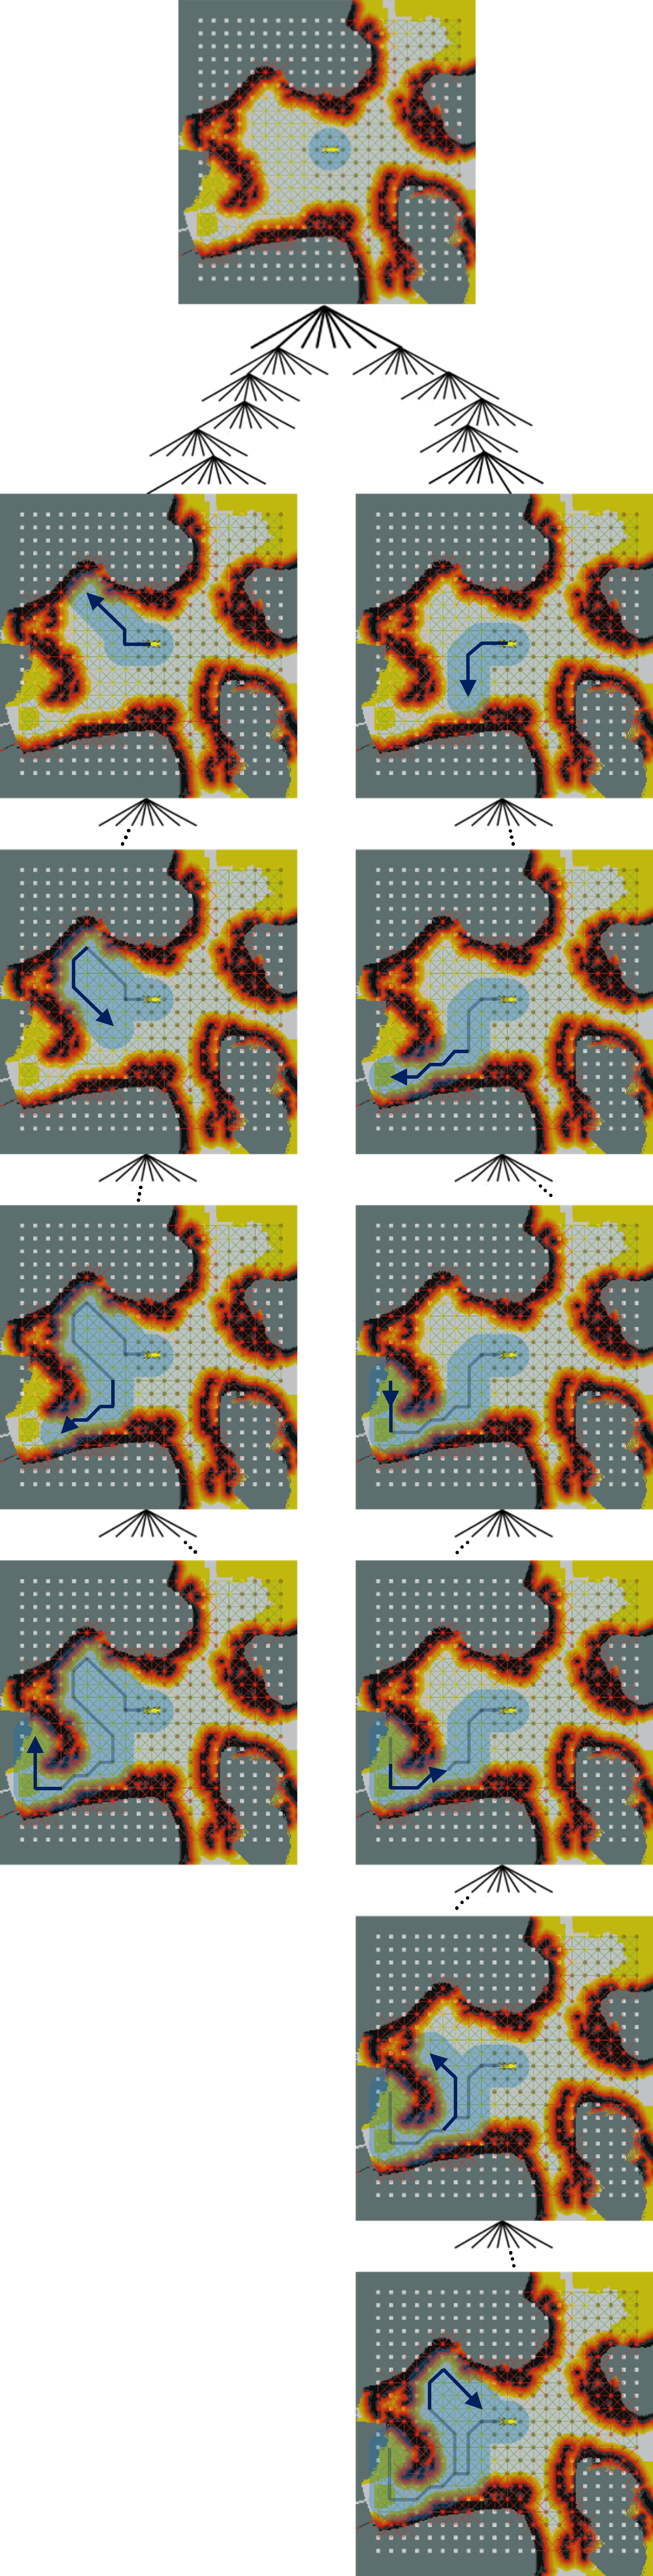
\includegraphics[width=0.25\textwidth]{figures/tree_figure_cropped_paths4.png}};
% 	    \begin{scope}[x={(image.south east)},y={(image.north west)}]
% 	    
% 	   % 	% Annotations [Time]
% 	   % 	\node [font=\scriptsize,above left,align=right,white] at (0.245,0.58) {0.00 s};
% 	   % 	\node [font=\scriptsize,above left,align=right,white] at (0.495,0.58) {11.8 s};
% 	   % 	\node [font=\scriptsize,above left,align=right,white] at (0.742,0.58) {4.33 s};
% 	   % 	\node [font=\scriptsize,above left,align=right,white] at (.992,0.58) {59.6 s};
% 	    	
% 	   % 	% Annotations [Scale]
% 	   % 	\node [font=\scriptsize,above left,align=right,black] at (0.044,0.045) {3 m};
% 	   % 	\node [font=\scriptsize,above left,align=right,black] at (0.8,0.05) {4.25 m};
%
% 	    \end{scope}
% 	\end{tikzpicture}	
% \caption{Tree Search} \label{fig:mlp_hardware_tests} 
% \end{figure}



% \begin{figure}[!t]
%   \centering
%   \subfloat[Coverage]{%
%     \includegraphics[width=0.53\columnwidth,trim={0 6.5cm 10.5cm 0},clip]{figures/s2_comparison.pdf}
%   }
%     \,
%   \subfloat[Plot]{%
%     \includegraphics[width=0.43\columnwidth,trim={15cm 8.3cm 3cm 0},clip]{figures/s2_comparison.pdf}
%   }
%   \caption{PLGRIM (top, across) vs. NBV (bottom, across). From left to right, the progress of coverage at $t=30$s, $t=50$s, and $t=80$s.  Note that PLGRIM explores more compactly and efficiently than the NBV approach.}
%   \label{fig:station-baseline}
% \end{figure}
\begin{figure}[!t]
  \centering
  \subfloat[Snapshots of autonomous exploration in wide-oepn space. Dark yellow region indicates the covered area by the robot.]{%
    \includegraphics[width=1.0\columnwidth,trim={0 7.5cm 10.5cm 0},clip]{figures/s2_comparison.pdf}
  }
  \\
  \subfloat[Plot of covered area over time.]{%
    % \includegraphics[width=0.6\columnwidth,trim={15cm 8.4cm 3cm 0},clip]{figures/s2_comparison.pdf}
    \includegraphics[width=0.6\columnwidth]{figures/subway_station_coverage.png}
  }
  \caption{PLGRIM (top, across) vs. NBV (bottom, across). From left to right, the progress of coverage at $t=30$s, $t=50$s, and $t=80$s.  Note that PLGRIM explores more compactly and efficiently than the NBV approach.}
  \label{fig:station-baseline}
\end{figure}


In Fig.~\ref{fig:station-baseline}, shows the quantitative results during the autonomous exploration mission.
% (More experimental results will come.)

% \begin{figure}[!t]
  % \centering
  % \subfloat[Hardware Testing]{%
    % \includegraphics[width=.45\columnwidth]{figures/subway_station_coverage.png}
  % }
  % \caption{Total distance traveled (blue), total area covered (purple), and the number of sectors on the environment (red) versus  time.}
  % \label{fig:may-demo-plot}
% \end{figure}


\subsection{Hardware Results}


\begin{figure*}[h!]
\centering
    \begin{tikzpicture}
	    \node[anchor=south west,inner sep=0] (image) at (0,0) {\includegraphics[width=1\textwidth]{figures/mlp_figure_scale.png}};
	    \begin{scope}[x={(image.south east)},y={(image.north west)}]
	    
	    	% Annotations [Letters]
	    	\node [above left,align=right,white] at (0.035,0.91) {A};
	    	\node [above left,align=right,white] at (0.28,0.91) {B};
	    	\node [above left,align=right,white] at (0.53,0.91) {C};
	    	\node [above left,align=right,white] at (0.78,0.91) {D};
	    
	    	% Annotations [Time]
	    	\node [font=\scriptsize,above left,align=right,white] at (0.245,0.58) {5:08};
	    	\node [font=\scriptsize,above left,align=right,white] at (0.495,0.58) {5:20};
	    	\node [font=\scriptsize,above left,align=right,white] at (0.742,0.58) {5:24};
	    	\node [font=\scriptsize,above left,align=right,white] at (.992,0.58) {6:24};
	    	
	    	% Annotations [Scale]
	    	\node [font=\scriptsize,above left,align=right,black] at (0.044,0.045) {2 m};
	    	\node [font=\scriptsize,above left,align=right,black] at (0.787,0.045) {2 m};

	    \end{scope}
	\end{tikzpicture}	
\caption{MLP} \label{fig:mlp_hardware_tests} 
\end{figure*}


\begin{figure*}[h!]
\centering
    \begin{tikzpicture}
	    \node[anchor=south west,inner sep=0] (image) at (0,0) {\includegraphics[width=1\textwidth]{figures/glp_figure_processed}};
	    \begin{scope}[x={(image.south east)},y={(image.north west)}]
	    
	    	% Annotations [Letters]
	    	\node [above left,align=right,white] at (0.035,0.91) {A};
	    	\node [above left,align=right,white] at (0.28,0.91) {B};
	    	\node [above left,align=right,white] at (0.53,0.91) {C};
	    	\node [above left,align=right,white] at (0.78,0.91) {D};
	    	
	    	% Annotations [Time]
	    	\node [font=\scriptsize,above left,align=right,white] at (0.245,0.58) {09:11};
	    	\node [font=\scriptsize,above left,align=right,white] at (0.495,0.58) {10:36};
	    	\node [font=\scriptsize,above left,align=right,white] at (0.742,0.58) {12:26};
	    	\node [font=\scriptsize,above left,align=right,white] at (.992,0.58) {14:16};
	    	

	    \end{scope}
	\end{tikzpicture}	
\caption{GLP} \label{fig:mlp_hardware_tests} 
\end{figure*}



% Coverage at time t
% : 4m FOV, following the robot traj, compute the total sweeping area

% Local IRM sweeping at time 0:t
% : 20m FOV, following the robot traj, compute the total reachable sweeping area

% relative coverage = Area(C) / Area(L)



%%%%%%%%%%%%%%%%%%%%%%%%%%%%%%%%%%%%%%%%%%%%%%%%%%%%%%%%%%%%%%%%%%%%%%%%%%%%%%%%
\section{Conclusion}\label{sec:conclusion}

% POMDP in reality
% - overcome challenges
%   : curse of dimensionality
%     . multi-resolution uncertainty representation
%     . cascaded hierarchical planning
%   : curse of history
%     . receding horizon planning
%     . resilience and consistency for unknown environment exploration with MPC
% - benefit
%   : non-myopic decision making, unlike frontier-based exploration --> less oscillation, better performance
%   : scalable framework for dense coverage motion planning with large-scale global coverage completeness
% - results
%   : sim/hw experiments


In this work, we have developed a hierarchical framework for exploring large-scale unknown environments in a POMDP setting. 
To obtain a tractable solution we discretize the belief space into a robot and task-relevant graph structure which reduces our search space for good policies.
The hierarchical planning framework and formalization of the unified optimal policy enabled scaling up the highly complex coverage problems.
We demonstrate these capabilities in the high-fidelity dynamic simulation environment.  

The future work includes learning-based methods for graph expansion information gain estimation, and a richer incorporation of risk and time into the graph planning framework.
Another interesting venue is the extension of this framework to the multi-robot coverage problems.


% \clearpage{}

%%%%%%%%%%%%%%%%%%%%%%%%%%%%%%%%%%%%%%%%%%%%%%%%%%%%%%%%%%%%%%%%%%%%%%%%%%%%%%%%
\bibliographystyle{aaai21}
\bibliography{references}  % .bib



%%%%%%%%%%%%%%%%%%%%%%%%%%%%%%%%%%%%%%%%%%%%%%%%%%%%%%%%%%%%%%%%%%%%%%%%%%%%%%%%
\appendix
\section{Appendix: Detailed Hierarchical Planner Instantiation}\label{sec:appendix}

In this section we present the detailed description of the POMDP-based coverage planner at each hierarchical level.


% \subsection{Overall Framework} 

% % \begin{figure}[t!]
% %   \centering
% %   \includegraphics[width=.6\textwidth]{figures/SystemOverview.png}
% %   \caption{[WIP] System overview}
% %   \label{fig:system_overview}
% % \end{figure}

% FIGURE: System Diagram
% Input source to Graph-level Planner and Lattice-level Planner 
% Connection between GLP and LLP
% (move\_base)-level motion planner

% ?? NEED TO MENTION SLAM MODULE??


% See \url{https://docs.google.com/presentation/d/1DfS1T1_o_xenJ4o8x-9D0Uq-EO1xwyToqdSEE_V9eyU/edit#slide=id.g8cd3872972_2_0} for figure draft.


\subsection{Graph-Level Planner} 

% pseudo code

\ph{Environment Representation} We employ a sparse bidirectional graph structure $G^g = (V^g, E^g)$ that captures the connectivity of the free space in the environment. We refer to this graph as the information roadmap (IRM) as its nodes $V^g$ and edges $E^g$ are enriched with environmental information. Each node $v^g \in V^g$ has attached to it a feature vector containing the probability $p(occ(v^g))$ that the node is occupied and the probability $p(cov(v^g))$ that the node has been sensed by the robot. Likewise, each edge $e_{ij}^g \in E$ has attached to it a feature vector containing the probability $p(\rho(v_i^g, v_j^g)$) of traversal between the connected nodes $v_i^g$ and $v_j^g$.

\ph{State} Two-tuple $s^g=(G^g, Q^g) \in \mathbb{S}$ consisting of the current graph state $G^g$ and the robot state $v_q^g$ defined as the node closest to the robot's position. 

\ph{Graph action information reward}
We can approximate the graph action information reward $I^g(v, \pi^g)$ by the number of unknown cells within a 5m radius of the goal node $\pi^g(v_i)=v_j$.  This is an effective approximation when we assume a perfect sensor model which changes the probability of occupancy from 0.5 to either 1 or 0.  

\ph{Observation} The observation $z \in \mathbb{Z}$ received by the robot are the nodes directly connected to node $v_q$. The observation model is defined as $O: V^{cov} \times S \rightarrow \mathbb{Z}$ where $S$ is one edge length.

% \ph{Action} Defined in "Abstract Planner"

\ph{Transition Model} We define the output of the graph policy $\pi^g(v_i^g)$ to be a neighboring node $v_j^g$, which is connected via a short path through free space. We assume that $\pi^{g}(v_i^g)$ induces a transition from nodes $v_i^g$ to $v_j^g$ with probability one:
\begin{align}
    T^{g} (v_i^g, \pi^g(v_i^g), v_j^g) = 1
    s.t.~&~\rho(b_t^g,\pi(b_t)) < \psi(t)
\end{align}

The acceptable risk threshold $\psi(t)$ is time-varying. As the duration of the mission progresses, the risk threshold $\psi(k)$ can increase to allow for riskier actions.

\ph{Observation}

\ph{Reward} We define the graph reward as the reward gained by executing the graph-level policy $\pi^g$ from node $v$ as a function $R^g(v, \pi^g): V \times \Pi^g \to \mathbb{R}$. The reward function, as defined in Eq. (\ref{eq:reward}), includes costs associated with path length and risk and utility associated with the observation $z$ of previously uncovered nodes. 

% The IRM graph grows through the addition of new nodes and edges as the robot navigates to previously unexplored areas of the map. We distinguish between two types of nodes: breadcrumb nodes and frontier nodes. Roughly speaking, breadcrumb nodes $b\in B \subset V$ encode the connectivity of free and traversable (low risk) space where the robot has previously explored, and frontier nodes $f\in F\subset V$ encode additional information about the value of exploring new locations, with $F\cup B = V$.

\subsection{Lattice-Level Planner} 

\ph{Environment Representation} We employ a rolling, fixed-sized lattice structure $G^\ell = (V^\ell, E^\ell)$ which is centered at the robot's current position. For ease of notation, we will drop the lattice notation for the remainder of this section. Each node object $v \in V$ has attached to it a feature vector containing the node position, probability of occupancy $p_{occ}(v)$, and probability $p_{cov}(v)$ that the node has been sensed by the robot. 

\ph{Risk} Each edge object $e \in E$ contains a risk value, or the probability of failing to safely traverse from node $v_i$ to connected node $v_j$:
\begin{align}
    \rho_{ij}(V; W_{occ}) = \mathcal{F} \big(v_i, \, v_j; \, p(W_{occ})\big)
\end{align}
where $W_{occ}$ encodes the 3D volumetric occupancy information acquired from raw sensor data. Within each grid cell $w_i \in W_{occ}$, there may exist multiple risk factors, due to a different source of potential failure, including rough terrain, proximity to obstacles, slope, slippery/muddy terrain. The number of risk factors is denoted by $n_\rho$. We compute the probability of failing to traverse a cell $\rho_c(w_i)$ as:
\begin{align}
    \rho_c(w_i) = 1-\prod_{r=1}^{n_\rho} (1-\rho_r(w_i))
\end{align}
We then compute the risk of the entire path from node $v_i$ to node $v_j$ as the aggregate risk of traversing the cells along the path:
\begin{align}
    \rho_{ij} = 1-\prod_t^{t+\tau}(1-\rho_c(w_{i_t}))
\end{align}


\ph{State} Two-tuple $s=(G, Q)  \in \mathbb{S}$ consisting of the current lattice state $G$ and robot state $V_q = (v_q, \dot{v}_q)$ where $v_q \in V$ is the node representing the robot's position and $\dot{v}_q$ is the robot's velocity. 

\ph{Observation} The estimated observation $z \in \mathbb{Z}$ consists of the nodes within line-of-sight of the robot node $v_q$, computed using ray-casting techniques on the prior occupancy map $W_{occ}$ in conjunction with sensor range constraints:
\begin{align}
    w_{cov} = \hat{O}(V, q; \, W_{occ,0}) 
\end{align}

\ph{Action} The output of the lattice policy is a control input $\vec{u}$ to the robot. 

\ph{Transition Model} We define the output of the lattice policy $\pi(v_i)$ to be a neighboring node $v_j$, which is connected by edge $e_{ij}$. We assume that $\pi(v_i)$ induces a transition from nodes $v_i$ to $v_j$ equal to the probability of traversal:
\begin{align}
    \hat{T}^{g} (v_i, \pi(v_i), v_j) = \begin{cases} 
    1-\rho_{ij} \; &\text{if $\rho_{ij} < \psi(t)$}\\
    0 \; &\text{otherwise}
    \end{cases}
\end{align}
The acceptable risk threshold $\psi(t)$ is time-varying. As the duration of the coverage mission progresses, the risk threshold $\psi(k)$ can increase to allow for riskier actions.

\ph{Information Gain} Entropy is a measure for the uncertainty of a posterior. The entropy $H_p(x) = E[-\log p(x)]$ is the expected information that $x$ contains if $x$ happens with probability distribution $p$. The posterior uncertainty of the lattice structure is:
\begin{align}
    H_{p_{cov}}(V) =& 
    -\sum_{v_i \in V} \left[ p_{cov}(v_i) \log p_{cov}(v_i) + \right. \nonumber \\
      & \left. \left(1-p_{cov}(v_i)) \log (1-p_{cov}(v_i)\right) \right]
\end{align}
where $V$ is the set of nodes in the lattice, $v_i$ is the random variable associated with the $i$-th node, and $p_{cov}(v_i)$ is the probability that the node has been observed by the robot. The uncertainty reduction, or information gain, associated with an action $\pi(v_i)$ in belief $p_{cov}(V)$ is:
\begin{align}
    % I(\pi(v_i), w_{cov}) &= H_{p_{cov}}(V) - H_{p_{cov}}(V^\prime; \pi(v_i), w_{cov}) \\
    I(V; \pi(v_i), w_{cov}) &= \underbrace{H_{p_{cov}}(V)}_\text{current entropy} - \underbrace{H_{p_{cov}}(V^\prime; \pi(v_i), w_{cov})}_\text{future entropy}
\end{align}
where the second term represents the expected future entropy of the lattice when the agent observes $z = w_{cov}$ after executing action $\pi(v_i)$. The successor world state $p_{cov}(V^\prime)$ is computed according to Bayes' Algorithm (Eq. \ref{eq:belief_update}). 

\ph{Cost of Traversal} The cost of traversal associated with action $\pi(v_i)$ comprises risk, rotation, and traversal distance:
\begin{align}
    C(V; \pi(v_i), W_{occ}) = \alpha_{risk} \; \rho_{ij} + \alpha_{rot} \;  \cos^{-1}(\dot{\vec{v}}_q, \cdot \vec{u}) + \alpha_{dist} \; \vec{u}
    \label{eq:traversal_cost}
\end{align}
To account for the distance discrepancy between a lateral and diagonal action, we define $\alpha_{dist}=1$ if $\vec{u}$ is a multiple of $\pi/2$ (lateral action) and $\alpha_{dist}=\sqrt{2}$ (diagonal action) otherwise.

% (-pi, pi]
% [-135, -90, -45, 0, 45, 90, 135, 180]

% rotation penalty: $f(\dot{\vec{v}}_q, \vec{u}) = \cos^{-1}(\dot{\vec{v}}_q, \cdot \vec{u})$

% $Q^\ell = \{q, \dot{q}\}$
% $q \in \mathbb{V}$



\ph{Reward Function} The one-step estimated reward is a weighted sum of information gain and traversal cost:
\begin{align}
    % \hat{R}(s, a) : Q^\ell \times (W_{cov} \times \mathbb{Z}) \rightarrow \mathbb{R} \\
    \hat{R}(s, \pi(v_i)) = c_{I} I(V; \pi(v_i), w_{cov}) - c_{T}  C(V; \pi(v_i), W_{occ})
    \label{eq:lattice_reward}
    % \hat{R}(s, a) = c_{I} I(V; z) - c_{T} Cost()
\end{align}


% \subsection{Algorithm: NAME?? PLGRIM: Planning at Local and Global levels with Robust Information Maps}

% Here we explain how the two instances of abstract coverage planners (graph-level and lattice-level planners) are combined and interact with each other in a unified framework...

% Receding horizon control



% \subsubsection{Global Level}
% World represented as a graph. W = Simple bidirectional graph

% $s^g = (Q^g, G^g)$. $G^g \sim W?$. Here, $Q^g$ = robot node $q \in V^g$ vertices  and $\dot{q}$ is velocity vector.

% Generative model $\mathcal{G}$ is explained.

% Rollout policy $\pi_{rollout}$ is random or Dijkstra-based to reach next unexplored node

% Output of GLP is $\theta^\ell_t$, which gives a goal position to the robot executive (mobility service) to move the robot to an unexplored area of the map.

% \subsubsection{Local Level}
% World represented as a lattice. World W = dense lattice with occupancy information, similar to occupancy grid maps.

% Gl = hyperlocal coverage information in the lattice (within robot FOV). Here, Qg = robot node $v_q$  and unit velocity vector $\dot{v}_q$. 

% Generative model $\mathcal{G}$ is estimated from robot sensors. It assumes perfect motion model. It gives output $(s', o, r)$. Next state s' contains the new robot pose and velocity vector; . Observation o contains the occupancy information of lattice nodes within FOV of robot. r contains reward -- this includes fixed penalty for each step moved, distance penalty for moving along an edge, rotation penalty for change in robot velocity vector.

% Rollout policy $\pi_{rollout}$ is Dijkstra-based to reach next unexplored node

% Output of GLP is $a^{*l}_{t:T}$, which is a series of robot poses to reach, given to the robot executive.

% \subsubsection{Executive}
% Describe mobility services here. What info does it need to move to a new position?

% Goal position

% cost/risk maps

% other stuff?




\clearpage{}

\section{Exploratory Covering Salesman Problem}
\label{sec:ECSPasPOMDP}
In this section, we introduce the coverage problem as a variant of the traveling salesman problem, and show how we formalize it as a POMDP. We then discuss the challenges and our approach. %how the exact solution to this problem can easily become intractable.  

\ph{Covering Salesman Problem (CSP)} Given a known environment represented by an abstract graph structure $W = (V, E)$, with free and occupied nodes $V_{free}\cup V_{occ} = V$, the traditional coverage problem aims to find a sequence of nodes and edge traversals that pass through all free nodes $V_{free} \subseteq V$.  By incorporating a sensor field-of-view $F:V\rightarrow \mathcal{P}(V)$, which maps each node to a subset of "visible" nodes, and adding the objective of minimizing travel distance, the coverage problem can be seen as a generalization of the traveling salesman problem -- the \emph{covering salesman problem} (CSP).  In the CSP, the objective is to determine the minimum length path through a subset of nodes $\{v_i\}_i \subseteq V_{free}$ such that every free node is within the accumulated sensor field-of-view: $V_{free} \subseteq \cup_i F(v_i)$.
In this paper, we further modify the CSP by assuming that the environment $W$ is not known a priori, which we call an \emph{exploratory covering salesman problem} (ECSP).  After incorporating a consideration of motion and sensing uncertainty of the agent, we can cast the ECSP as a POMDP problem with a reward function designed for coverage, which we will refer to as \emph{ECSP-POMDP} hereafter.

\ph{ECSP-POMDP Elements} A POMDP is described as a tuple $\langle \mathbb{S}, \mathbb{A}, \mathbb{Z}, T, O, R \rangle$, where $\mathbb{S}$ is the set of states of the agent and world, $\mathbb{A}$ and $\mathbb{Z}$ are the set of robot actions and observations. At every time step, the agent performs an action $a \in \mathbb{A}$ in state $s$ and receives an observation $z \in \mathbb{Z}$ resulting from the agent's perceptual interaction with the environment. The motion model $T(s, a, s') = P(s'\,|\,s, a)$ defines the probability of being at state $s'$ after taking an action $a$ in state $s$. The observation model $O(s, a, z) = P(z\,|\,s, a)$ is the probability of receiving observation $z$ after taking action $a$ in state $s$. The reward function $R(s,a)$ returns the expected utility for executing action $a$ in state $s$.

\ph{State} We define the system (robot-world) state as a 2-tuple $s = (W, Q) \in \mathbb{W}\times\mathbb{Q} =  \mathbb{S}$ consisting of the robot state $Q$ and the regions of the world have been observed (covered) by the robot $W$. The world representation can be further decomposed as $W = (W_{occ}, W_{cov})$ where $W_{occ}$ describes a representation of the geometry of the world, and $W_{cov}$ encodes which regions of the world have been observed by the robot.  For example, $W_{occ}:\mathbb{Q}\rightarrow\{0,1\}$ can be a mapping from pose to the set $\{0,1\}$, where $W_{occ}(Q) = 0$ if the location is free and $W_{occ}(Q) = 1$ if the location is occupied (and similarly for $W_{cov}$).  We also denote the ground truth occupancy of the world as $W_{occ}^{GT}$.
% The underlying ground truth (complete) world is denoted by $W_{occ}$. For example, $W_{occ}:\mathbb{Q}\rightarrow\{0,1\}$ can be a binary mapping, where $W_{occ}(Q) = 0$ if the location is free and $W_{occ}(Q) = 1$ if the location is occupied (and similarly for $W_{cov}$).  %We also denote the ground truth occupancy of the world as $W_{occ}^{GT}$.

\ph{Belief State} Since the state of the world is not fully observable, the agent maintains a belief state $b_t\in \mathbb{B}$ defined as the posterior distribution over all possible states conditioned on past actions and observations at time $t$. The belief over state $s$ is $b_{t} = P(s \,|\, a_{0:t-1}, z_{1:t})$. The ESCP belief state is a 2-tuple $b_t = p(s_t) = p(W,Q)$.

\ph{Transition Model} Given an action $a$, the estimated transition model $T$ maps the robot and world state $s = (W, Q)$ to the subsequent state $s' = (W', Q')$, i.e., $T(s, a, s'; \, W_{occ}^{GT})$. 
The transition model is parameterized by ground truth world map $W_{occ}^{GT}$, which represents the generative model (in simulation or physical robot motion). %It encodes the traversability risk of an action $a \in \mathbb{A}$. 
The model $W_{occ}^{GT}$ encodes the true traversability information and determines if the robot can or cannot transition along the edge $e$ induced by action $a$.% and, consequently, the state does not change: $s = s'$.

\ph{Observation} Upon taking an action $a$ in state $s$, the robot receives an observation of the robot state $Q$ and a partial observation of the world state $W$. Given a robot state $Q$, the robot observes areas of the world within the field-of-view of its sensors.  The observation model is denoted by $  O(z | s, a; \, W_{occ}^{GT})$
where $O$ provides information about $W_{cov}$.% within the field-of view, which depends on a ray-casting model.

\ph{Traditional Map Representation} Grid maps are a common representation of the world state $W$ in robotics. %(which we introduced as having a continuous domain, i.e. $W:\mathbb{Q}\rightarrow \{0,1\}$)
By using grid cells $\bar{W}=\{m_i\}_i$ where $m_i$ represents the world state (occupancy, coverage, etc.) at the $i$-th cell, the world state is reduced to a discrete domain.  In this work, we lightly assume the presence of a mapping and costmap-generating module which creates a local map $\bar{W}$.  
In order to compute the posterior probability $p(\bar{W} | z_{1:t}, Q_{1:t})$ of the whole map $\bar{W}$, given the robot's measurements $z_{1:t}$ and trajectory $Q_{1:t}$, the binary cell states are traditionally approximated by assuming full independence between them \cite{TBF05,elfes1990stochastic}. Note that in this work, the resolution of $\bar{W}$ is about of 10cm for a 1m-sized robot.

\ph{Pose Graph} In addition to the grid map representation of the environment, we employ a \textit{pose graph} \cite{thrun2002probabilistic}, where $\mathcal{PG} = p(Q_{0:t})$ is the belief over the path history taken so far.  This pose graph is generated by a SLAM algorithm and should run in realtime to support our planning architecture.  %In practice we may simplify our representation of $\mathcal{PG}$ by approximating it with the maximum likelihood estimate.

\ph{Reward} The one-step reward is computed as a function of the information gain and cost associated with an action:
\begin{align}
    {R}(s, a) = \mathcal{F}\Big[\, \textit{InfoGain}(W_{cov}, z), \; \textit{Cost}(W_{occ}, a) \, \Big]%: \, \mathbb{S} \times \mathbb{A} \rightarrow \mathbb{R} 
\end{align}
Information gain is defined as the marginal gain of information: $\textit{InfoGain}(W_{cov}, z) = I(W_{cov} \cup z) - I(W_{cov})$, since the benefit of being in a state $s$ is dependent on whether the robot has already observed neighboring areas in the world. The cost of an action $Cost(W_{occ}, a)$ is a function of the world geometry $W_{occ}$ since this sub-state informs both the required actuator output (path length and velocity) and the proximity to the actuator's limitations (traversability risk) required to execute an action.

\ph{ESCP-POMDP} We define a belief policy as a function $\pi : \mathbb{B} \rightarrow \mathbb{A}$ which maps each belief state $b$ to an action $a$.  Let the belief reward $r(b,a)=\int_s R(s,a)b(s)ds$ be the expected reward of taking action $a$ at belief $b$.  The optimal policy maximizes the expected discounted sum of future rewards.
\begin{align}
  \pi^*(b) &= \arg\max_\pi \, \mathbb{E} \sum_{t=0}^{L} \gamma^t r(b_t, \pi(b_t)) 
  \label{eq:optimal_policy}
\end{align}
where $\gamma \in (0,1)$ is a discount factor which ensures that immediate rewards have a greater effect on decisions than future rewards. The overall objective is to solve this optimization problem in a computationally tractable way.

\ph{Intractability} 
%Given the high-dimensional grid representation of the world state, 
Eq. (\ref{eq:optimal_policy}) is a highly intractable optimization for large environments. This is because of 1) the high dimension of the belief state $b$, particularly with respect to the belief over the high-dimensional grid representation of the world state $\bar{W}$, and 2) the large timescale $L$ as the complexity of the search space grows exponentially with time. In the next section, we discuss our approach to further decompose and address this problem.




\clearpage{}
%%%%%%%%%%%%%%%%%%%%%%%%%%%%%%%%%%%%%%%%%%%%%%%%%%%%%%%%%%%%%%%%%%%%%%%%%%%%%%%%
\section{PLGRIM: Hierarchical Coverage Planning on Information Roadmaps}
\label{sec:plgrim}

% IRM construction: frontiers?

%\ph{Our Contributions} 
To obtain a tractable solution to the ESCP problem in Eq. (\ref{eq:optimal_policy}), we propose a novel approach in which we 1) introduce a hierarchical approximation of the belief space $b=p(W,Q)$ to reduce the policy search space, and 2) introduce a hierarchical POMCP solver to quickly find non-myopic solutions on local to global scales in real-time.

\ph{Architecture}  We decompose the problem into tractable subproblems by introducing spatial and temporal abstraction which enable efficient and reactive robot behaviors on very large scales (kms).  The hierarchical planner has two cascaded layers with different environment representation scales. The higher layer, which we call a \emph{graph-level planner}, employs a sparse graph structure of dynamic size which captures the connectivity of the free space in the known part of the environment. The lower layer, which we call a \emph{lattice-level planner}, employs an agent-centered dense grid structure of fixed dimensions that moves with the robot (see Fig.~\ref{fig:system_overview}). %6

\subsection{Hierarchical Belief Space Representation} 

\ph{Belief Encoding} Both the graph-level planner and lattice-level planner use a graph-based abstraction of the world state $W$.  We call these graph-based approximations an \textit{Information Roadmap (IRM)}. %\cite{agha2014firm}.
We use super-scripts $(\cdot)^g$ or $(\cdot)^\ell$ as needed to describe objects specific to the graph-level or lattice-level respectively. We describe the graph-level IRM first, but most discussions apply to the lattice-level IRM too. Let $V^g=\{v_i\}_i$ denote a set of robot poses $v_i\in \mathbb{Q}$.  Then for each pose $v_i\in V^g$ we construct an approximation of $W(v_i) \approx W^g(v_i)$, with $W_{occ}^g(v_i) = \{0,1\}$ and $W_{cov}^g(v_i) = \{0,1\}$.  %This approximation can be constructed by finding the maximum value $W_{occ}(v_j)$ for all $v_j$ in a neighborhood of $v_i$, or some other approximate method.  We also can approximate $W_{cov}^g$ as a function of the poses $V^g$ and the pose graph $\mathcal{PG}$. 
For details on computing these approximations for both graph-level and lattice-level, see the supplemental material.  We then construct an approximate graph-level belief $b^g=p(W^g, Q)$.  By assuming independence between variables, this belief can be decomposed as $b^g=p(Q)\prod_i p(W_{occ}^g(v_i))$.  Additionally, to create a meaningful decomposition of the action space, we construct edges $E^g=\{e_{ij}\}_{i,j}$ which connect the nodes $v_i, v_j$.  In doing so, we create a graph structure $G^g=(V^g, E^g)$ representation of the world.  We associate to the edges transition probabilities as well as other quantities of interest (e.g. risk, cost of traverse, etc).

Fig. \ref{fig:system_overview} illustrates the process by which the 3D volumetric information $W$, acquired from raw sensor data, is approximated into discrete probability distributions over occupancy and coverage. 
Therefore, we have approximated and discretized the belief space $b^g\in\mathbb{B}^g\subset\mathbb{B}$ and $b^\ell\in\mathbb{B}^\ell\subset\mathbb{B}$ for the graph and lattice-level planners to act on.

%\ph{POMDP Specifics}
For each planning problem in the hierarchy we define a sub-POMDP problem over the graph representation.  The details of these problems differ in terms of the definitions for transition models $T^g(\cdot),T^\ell(\cdot)$, observations $O^g(\cdot),O^\ell(\cdot)$, and rewards $R^g(\cdot),R^\ell(\cdot)$.  We detail the particular design choices used in this work in the supplementary material, and give the general framework here.

\subsection{Hierarchical Policy Formulation}
\label{sec:hierarchical_policy}
\ph{Policy} We define a graph-level policy as a mapping from the graph-level belief state $b^g$ to a goal-related parameter $\theta^g \in \Theta^g$ 
\begin{align}
    \pi^g : \mathbb{B}^g \to \mathbb{A}^g, \; \mathbb{A}^g = \Theta^g\ .
\end{align}
The action space $\Theta^g$ encodes a global, non-myopic task, and serves as an input to the lattice-level policy: 
\begin{align}
    \pi^\ell: \mathbb{B}^\ell \times \Theta^g \to \mathbb{A}^\ell\ .
\end{align}
The output of the lattice-level policy is a controller to move the robot (e.g. a waypoint or path for a controller to track, or parameters for a feedback policy that generates control commands).

We define an overall policy $\pi \in \Pi$ generated by combining the graph-level policy $\pi^g$ and the lattice-level policy $\pi^\ell$:
\begin{align}
    \pi(b) = \pi^\ell(b^\ell; \, \pi^g(b^g)) = \pi^\ell(b^\ell; \, \theta^g) : \, \mathbb{B}\rightarrow \mathbb{A} 
\end{align}

\ph{Reward} The one-step reward received by the agent upon taking a lattice-level policy $a^\ell$ in belief $b^\ell$ is:
\begin{align}
    r^\ell(b^\ell, a^\ell) = r^\ell(b^\ell, \pi^\ell(b^\ell; \theta^g) = r^\ell(b^\ell, \pi^\ell(b^\ell; \pi^g(b^g)))
    \label{eq:reward}
\end{align}

\ph{Policy} We define the hierarchical policy of the graph and lattice level policies as:
\begin{align}
  \pi^{*}(b) &= \arg\max_\pi \, \mathbb{E} \left[ \sum_{t=0}^{L} \gamma^t r^\ell(b^\ell_t, \pi^\ell(b^\ell_t; \pi^g(b^g_t)) \right]
  \label{eq:optimal_policy_unified}
\end{align}

\ph{Policy decomposition and interaction} In this work, we choose to represent the graph planner's output actions $\theta^g$ as nodes $v^g_i \in V^g$ in the graph-level IRM $G^g$. These nodes are passed to the lattice planner, whose objective is to explore locally. Similarly, the lattice-level planner's output actions are nodes $v^\ell_i \in V^\ell$ in the lattice-level IRM $G^\ell$.  In order to maintain a tractable problem in both the graph and lattice levels, we decouple the policies in the following manner:  The lattice-level planner typically sends its action $v^\ell_i$ to the kinodynamic planner, which produces velocity commands for the robot.  However, if there is no exploration possible in the lattice map, the lattice-level planner passes along the graph-level planner's action $v^g_i$ to the kinodynamic planner, which encodes a new area in the graph-level IRM for the lattice-level planner to explore.  At any time the lattice-level planner may decide to continue exploring on the lattice-level IRM.  In this manner, we encourage high-fidelity local exploration without sacrificing large-scale, globally optimal decision making.

In the next section, we describe the POMDP solver approach to optimizing the global and local policies of Equation \ref{eq:optimal_policy_unified}.


%%%%%%%%%%%%%%%%%%%%%%%%%%%%%%%%%%%%%%%%%%%%%%%%%%%%%%%%%%%%%%%%%%%%%%%%%%%%%%%%
\subsection{Real-time Hierarchical Solver for ECSP-POMDPs}

% \textbf{Separate POMCP algorithm -- SIMULATE ROLLOUT SEARCH}



% Amanda/David Version
%%%%%%%%%%%%%%%%%%%%%%%%%%%%%%%%%%%%%%%%%%%%%%%%%%%%%%%%%%%%%%%%%%%%%%%%%%%%%%

\begin{algorithm}[t!]
\caption{Hierarchical Coverage Planner}
\label{alg:hierarchicalPlanner}
\begin{multicols}{2}
% \vspace{-10pt}
\begin{algorithmic}
\STATE \underbar{\textbf{Function HierarchicalPlan}}
\item \textbf{input: }Beliefs $b^g$, $b^l$ of states $s=(G, Q)$
\item \textbf{input: }World configuration $W$
% \item \textbf{input: }Optional rollout policy $\pi_{rollout}$
\REPEAT
    \STATE \textbf{\# Global planner}
    \item  Obtain world information map
    \item Estimate $\hat{\mathcal{G}}^g$
    \item $\theta^l_{t:T} \gets \textsc{POMCP}(b^g, \hat{\mathcal{G}^g}, \pi_{rollout})$
    \STATE \textbf{\# Local planner}
    \item Obtain local information map
    \item Estimate $\hat{\mathcal{G}}^l$
    \item $a_{t:T}^{*l} \gets \textsc{POMCP}(b^l;\hat{\mathcal{G}}^l, \theta^l_{t:T}, \pi_{rollout})$ 
    % \item \#learn value function and get best actions
    \STATE \textbf{\# Executive}
    \item Execute $a_{t:T}^{*l}$
    \item Obtain $z$ from sensors
    \item Update $Q$, $W$
\UNTIL timeout
\end{algorithmic}

\begin{algorithmic}
\STATE \underbar{\textbf{Function POMCP}}
\STATE \textbf{input: }Initial belief state $b_0$
\STATE \textbf{input: }Estimated generative model $\hat{\mathcal{G}}$
\STATE \textbf{input: }Optional rollout policy $\pi_{rollout}$
% \STATE
\STATE Initialize empty MCTS tree $T_r$
\REPEAT
    % \item Initial state $s_0 \sim b_0$
    \item \# Run SIMULATE with $\pi_{rollout}$ and $\hat{\mathcal{G}}$ to update $T_r$ with learned value function
    \item $T_r \gets \textsc{SIMULATE}(b_0; \hat{\mathcal{G}}, \pi_{rollout})$
    % \STATE Update the values and the number of visits by backpropagation from the leaf node to the root node
\UNTIL{timeout}
% \item 
\item Extract next N actions $a^*_{1:N}$ from $T_r$ \#N=1 for GLP. For LLP, keep going till leaf node
% \STATE
\RETURN $a*_{1:N}$
\STATE
\STATE
\STATE
\STATE
\end{algorithmic}

\end{multicols}
\end{algorithm}


\begin{figure*}[t!]
  \centering
  \includegraphics[width=0.8\textwidth]{figures/belief_tree_search_policy.pdf} % with an arrow
  \caption{Illustration of coverage planning with Monte-Carlo Tree Search. A state contains a coverage state of the environment $W$ and a robot pose $q$, and the current state is $(W_o, q_2)$. From forward simulation of possible action sequences and back-propagation of the rewards (e.g., information gain per traversal distance), it can find the best action for the current state, which is \texttt{move-to-$q_1$}.}
  \label{fig:belief-tree-search}
\end{figure*}



%\ph{Architecture}
Algorithm~\ref{alg:hierarchicalPlanner} outlines the overall PLGRIM framework for hierarchical coverage planning.  (See also Fig.~\ref{fig:system_overview}.)
At each replanning episode, both the graph-level and lattice-level planners employ a POMDP solver to find a policy at each level, $\pi^g$ and $\pi^\ell$.  To find these policies we employ POMCP, a Monte-Carlo Tree Search-based POMDP solver \cite{silver2010monte}.  This method requires only a generative model $\mathcal{G}$  (i.e., a black box simulator of the POMDP) instead of explicit mathematical models of the motion and sensing uncertainty. During each simulation, the initial state is sampled from the initial belief state, and the generative model provides a sample of the successor state $s'$, observation $z$, and reward $r$ based on the dynamics of the environment. However, the true state of the world $W^{GT}$ is unknown.  Thus, an approximate generative model $\hat{\mathcal{G}}^g$, $\hat{\mathcal{G}}^\ell$ is employed for each POMDP (graph and lattice) which uses a posterior distribution of the state  based on sensor data, $p(W^{GT}; a_{0:t-1}, z_{1:t})$ (omitting superscripts $(\cdot)^g, (\cdot)^\ell$):
\begin{align}
    \hat{\mathcal{G}}(\cdot) = \mathcal{F}(s, a; \, p(W^{GT}; a_{1:t}, z_{1:t})) = \mathcal{F}\big[T(\cdot), O(\cdot), R(\cdot)\big]%: \, \mathbb{S} \times \mathbb{A} \rightarrow \mathbb{S} \times \mathbb{Z} \times \mathbb{R}
\end{align}

As the robot moves through the environment, its sensors are used to update the pose-graph $\mathcal{PG}$ and the %kinodynamic 
costmap $\bar{W}$.  These are sent to modules which update the global-level IRM $W^g$ and the lattice-level IRM $W^\ell$, as well as estimates of the generative models $\hat{\mathcal{G}}^g$ and $\hat{\mathcal{G}}^\ell$. For details of these modules, see the supplemental material.

\ph{Implementation Details}
The POMCP solver uses Monte-Carlo Tree Search over the belief space of the world. Fig.~\ref{fig:belief-tree-search} shows a sample domain where the robot has covered parts of the world, shown in white. From node 2, the robot runs POMCP with the generative model $\mathcal{G}$, to generate the MCTS tree in the center of the figure. The red path (left) explores node $a$ first and then $c$, before moving onto node 5. The blue path (right) explores node $c$ first and then $a$, before moving onto 5. The solver simulates these sequences and back-propagates the rewards to output the optimal step (\texttt{move-to-$q_1$}) for the robot.

% (See Fig.~\ref{fig:belief-tree-search}). 


%%%%%%%%%%%%%%%%%%%%%%%%%%%%%%%%%%%%%%%%%%%%%%%%%%%%%%%%%%%%%%%%%%%%%%%%%%%%%%%%
\subsection{Receding Horizon Planning}
% Story
% Reward is from IG, IG from observations, Observations from robot motion execution 
% Robot motion execution depends on the robot state (heading, velocity, …) in the MPC layer
% If our next path is in the opposite direction of the current path, then it will take longer time…
% Consistent path over sequential coverage planning will increase the IG...
% ⇒ We should consider previous path in the current planning to guarantee consistency

Due to the nature of unknown space exploration with a limited field of view, the agent \ncomment{decision making} only has access to a part of the environment $W$ at anytime $t$. Hence, to fulfil its goal of exploration, we formulate the planning problem such that the agent gets reward from information gain (e.g. uncovering new regions).

This information gain is a metric we have designed \ncomment{learned?} from observations the robot has made \gautam{TODO: describe if needed}. These observations include sensor information such as accelerometers, motor encoders, \ncomment{images?} etc. The observations are gathered as the robot executes motion plans in the environment and forms a graphical representation with information stored mapped to the pose of the robot, known as the pose graph. \gautam{exclude this?}

Note that these plan executions are dependent on the robot state at the \textit{execution} layer, using Model Predictive Control. The heading and velocity of the robot at the end of a path can significantly affect the execution of the next path. Thus, during planning we have to consider the previous path the robot has taken as well, to ensure path consistency during exploration. Such a consistent path will increase the information gain per unit distance travelled \gautam{(or per unit time?)}.

Thus, the optimal exploration policy based on information gain (IG) is given by
\begin{align}
  \pi^*(IG) &= \arg\max_\pi \, \mathbb{E} \left[ \sum_{t=0}^{H} \gamma^t r(s_t, \pi(s_t)) \right]
  \label{eq:ig_policy}
\end{align}
where H is the finite horizon for planning

% suggestion from Sung
% One main point we want to show in MLP is the consistency + resilience (which may conflict to each other). Consistency is needed in general to make a smoother/full-speed motion of the robot (like 1->2). Resilience is needed when some obstacle pops up and path should be adaptively changed (like 2->3).
% we consider this conflicting objectives in our unified objective function. It would be great if we can formally present that.

Note, however, that a consistent path for the robot reduces it’s ability to react quickly to changes in the perceived map. This resilience could be required, for example, when the sensor readings from far away show a location as free, but when we come closer and collect more readings, it turns out to be an obstacle at close distance. Hence, we need to combine and weigh these aspects of the planner to make it both consistent and resilient in it’s planning.




\end{document}
